%%%%%%%%%%%%     Einstellungen      %%%%%%%%%%%%%%%%%%%%%%%%%%%%%%%%%%%%%%%%%%%%%%%%%%%%
%%%%%%%%%%%%%%%%%%%%%%%%%%%%%%%%%%%%%%%%%%%%%%%%%%%%%%%%%%%%%%%%%%%%%%%%%%%%%%%%%%%%%%%%

% Grundlegende Einstellungen
\documentclass[fontsize=10pt,openright,paper=a4]{scrbook}
\usepackage[bottom=4.0cm, left=3.0cm, right=3.0cm]{geometry} 
\usepackage[squaren, thinspace ,thinqspace]{SIunits}
\usepackage[latin2]{inputenc}
\usepackage[T1]{fontenc}
\newcommand{\changefont}[3]{
\fontfamily{#1} \fontseries{#2} \fontshape{#3} \selectfont}
%\changefont{pbk}{b}{sc}
\usepackage{lmodern}
\renewcommand*\familydefault{\sfdefault} %% Only if the base font of the document is to be sans serif
\usepackage[T1]{fontenc}
%\changefont{phv}{m}{n}
\usepackage{amsmath}
%\usepackage{amsfonts}
\usepackage{amssymb}
%\usepackage[english]{babel} % neue deutsche Rechtschreibung
\usepackage{graphicx}
%\usepackage{picins}
\usepackage{wasysym}
\usepackage{subfigure}
\usepackage{afterpage}
\usepackage{color}
\usepackage{float}
\usepackage{mathrsfs}
\usepackage{tabularx}
\usepackage{slashed}
%\usepackage{appendix}


\usepackage[small]{caption}
\usepackage[plainheadsepline,automark]{scrpage2}

\captionsetup{font={small}}

% Verlinktes Inhaltsverzeichnis
\usepackage[bookmarks=true, bookmarksnumbered=false,  
bookmarksopen=false,colorlinks=true,linkcolor=black]{hyperref}

\setlength{\parindent}{0mm}
% Header
\pagestyle{scrheadings}
% loescht voreingestellte Stile
\clearscrheadings
\clearscrplain
\automark[section]{chapter}

\setheadsepline{1pt}        %Separate Linie im Kopf
\renewcommand*{\chapterheadstartvskip}{\vspace*{1pt}} % Abstand vor Kapitel�berschriften

\ihead[]{\leftmark}
\ohead[]{\rightmark}
\ofoot[\pagemark]{\pagemark}

\cfoot[]{}

\author{Jan-Frederik Schulte}
\title{CMS Dilepton edge search}

%%%%%%%%%%%%%%%%%%%%%%%%%%%%%%%%%%%%%%%%%%%%%%%%%%%%%%%%%%%%%%%%%%%%%%%%%%%%%%%%%%%%%%%%
%%%%%%%%%%%%     Titelseite/Inhalt      %%%%%%%%%%%%%%%%%%%%%%%%%%%%%%%%%%%%%%%%%%%%%%%%
%%%%%%%%%%%%%%%%%%%%%%%%%%%%%%%%%%%%%%%%%%%%%%%%%%%%%%%%%%%%%%%%%%%%%%%%%%%%%%%%%%%%%%%%
%\changefont{pbk}{b}{sc}
%Dokument
\begin{document}


%Titelseite
\thispagestyle{empty}
\begin{center}
  ~ \\
  \vspace{-0.5cm}
 {\huge\bf{Search for Supersymmetry in opposite-sign same-flavour dilepton events with the CMS detector in proton-proton collisions at $\sqrt{s}=8$ TeV}\\}
  \vspace{2.5cm}
    { Von der Fakult\"at f\"ur Mathematik, Informatik und Naturwissenschaften der
RWTH Aachen University zur Erlangung des akademischen Grades
eines Doktors der Naturwissenschaften genehmigte Dissertation\\}
  \vspace{2.5cm}
    {\Large vorgelegt von}\\
    {\Large\bf Jan-Frederik Schulte, M.Sc.}\\
    {\Large\bf aus M\"unster } \\
    
  \vspace{3.cm}
    {\large Berichter: }\\
  	{\Large\bf Prof. Dr. Lutz Feld}\\
  	{\Large\bf Prof. Dr. Michael Kr\"amer}\\
  	
  \vspace{2.cm}
  {\Large Termin der m\"undlichen Pr\"ufung: xx.xx.2015\\}
  \vspace{2cm}
  {\Large Diese Dissertation ist auf den Internetseiten der Hochschulbibliothek online verf\"ugbar.}	
\end{center}
\cleardoublepage
\newpage
\newpage
\pagenumbering{roman}

%\addsec{Zusammenfassung}
%\input{Zusammenfassung}
%\addsec{Abstract}
%\input{Abstract}

%Inhalt
\tableofcontents
\clearpage

%%%%%%%%%%%%%%%%%%%%%%%%%%%%%%%%%%%%%%%%%%%%%%%%%%%%%%%%%%%%%%%%%%%%%%%%%%%%%%%%%%%%%%%%
%%%%%%%%%%%%     Hauptteil     %%%%%%%%%%%%%%%%%%%%%%%%%%%%%%%%%%%%%%%%%%%%%%%%%%%%%%%%%
%%%%%%%%%%%%%%%%%%%%%%%%%%%%%%%%%%%%%%%%%%%%%%%%%%%%%%%%%%%%%%%%%%%%%%%%%%%%%%%%%%%%%%%%
%
%
\pagenumbering{arabic}
\chapter{Introduction}
%The desire to understand the fundamental building blocks and underlying structures of our world has driven humanity's exploration of physics at the smallest scales. What started out as a pursuit of ideas purely within the mind in ancient Greece has developed into a fruitful interplay of both experiment and theory in modern particle physics. Today the Standard Model of particle physics describes the known particles and their interactions and has withstood countless experimental challenges. However, theoretical concerns and the desire to incorporate experimental observations not yet described within the Standard Model have lead to the conviction that yet unknown physical effects will manifest themselves if particle interactions are probed at energy scales of $\mathcal{O}$($\mathrm{TeV}$).

This is the purpose of the Large Hadron Collider (LHC), which collides protons at centre-of-mass energies of several $\mathrm{TeV}$. In addition to many precision measurements of established phenomena at this previously inaccessible energy scale, discovering the Higgs boson and thereby completing the Standard Model has been a large success of this undertaking. Now the focus lies even more on going beyond the Standard Model into the realm of new physics. Many ideas exists on how to extend the existing theory and an extensive search program is conducted in search of the new particles and interactions predicted by those models. 

One of the most attractive concepts is that of Supersymmetry, which introduces a symmetry between fermions and bosons. In this framework, a partner particle to each of the known Standard Model particles exists, differing in spin by $\frac{1}{2}\hbar$. In principle these partners have the same mass as their Standard Model counterparts. However, none of them have been discovered yet, which implies that Supersymmetry is broken, allowing for higher masses of the supersymmetric particles.

In this analysis, evidence for the existence of heavy supersymmetric particles is sought, exploiting a characteristic signature of their decay. In the decay of a neutralino particle, two charged leptons of the same flavour and opposite sign can be produced together with a lighter neutralino, which escapes detection. This correlated production of the leptons results in a characteristic edge in the distribution of their invariant mass.

The full data sample of proton-proton collisions at a centre-of-mass energy of 8\TeV recorded by the Compact Muon Solenoid (CMS) experiment in 2012, corresponding to an integrated luminosity of \lumi, is used. The presence of a supersymmetric signal in the data is assessed in two ways. First, event counts in different selections are compared to the expectation from Standard Model backgrounds. In a second approach, the characteristic edge signature is used in a shape analysis to separate a possible signal from the backgrounds. In the both cases, the background contributions are estimated entirely from data. 

This work builds upon the previous achievements by Nikals Mohr and Daniel Sprenger in their doctoral theses~\cite{Mohr:1423334,Sprenger:1501963} and has been performed in part in collaboration with Marco-Andrea Buchmann~\cite{Buchmann:1704399}. The results have been published by the CMS collaboration~\cite{Khachatryan:2015lwa}. This analysis presents an update of the published result, taking into account a later reprocessing of the data sample with improved calibrations. However, the analysis techniques have not been altered and the outcome of the analysis remains largely unchanged.

This thesis is structured as follows: The remainder of this section is dedicated to the definition of commonly used variables. Section~\ref{sec:theo} discusses the theoretical foundations relevant to the analysis. In Section~\ref{sec:setup} the LHC and the CMS detector are described. The methods used to analyse the recorded data are outlined in Section~\ref{sec:ana} and the estimation of Standard Model backgrounds from data is presented in Section~\ref{sec:backgrounds}. The results of the analysis in the two approaches discussed above are presented in Sections~\ref{sec:counting} and~\ref{sec:fit}. 

\section{Definition of variables}
\label{sec:variables}
Throughout this thesis, quantities are expressed in natural units. In this system, the speed of light and the reduced Planck constant are set to unity:
\begin{equation}
c = \hbar = 1.
\end{equation} 
Energies and momenta are measured in \GeV and lengths in $\text{\GeV}^{-1}$. However, sometimes lengths are also given in meters or centimeters, if convenient. 

The cross section of a physical process is given in barn, $\unit{1}{\barn}$ corresponding to $\unit{10^{-24}}{\centi\meter\squared}$.   

The CMS experiment uses a right-handed coordinate system where the x- and y-axis point perpendicular to the beam direction towards the center of the LHC and upwards, respectively. The z-axis points in the direction of the counter-clockwise beam.  These coordinates are usually transformed into a spherical coordinate system where $\phi$ is the azimuthal and $\theta$ is the polar angle. Instead of $\theta$ the pseudorapidity 
\begin{equation}
\eta = -\ln \left( \tan\left(\frac{\theta}{2}\right)\right)
\end{equation}
is commonly used, which coincides with the rapidity $y = \frac{1}{2} \ln\left(\frac{E+p_z}{E-p_z}\right)$ for $E\approx |p|$. The geometric distance of two objects in the detector is given by
\begin{equation}
\Delta R = \sqrt{(\phi_1 - \phi_2)^2 + (\eta_1 - \eta_2)^2}.
\end{equation}

As the collisions at hadron colliders involve interactions of partons carrying unknown fractions of the protons' momenta, the momentum of the initial state along the beam axis is unknown. As the momenta of the partons transverse to the beam are negligible compared to those in z direction, the transverse plane provides a well defined initial state. Therefore, the transverse momentum and energy
\begin{eqnarray}
\pt = \sqrt{p_x^2  + p_y^2} = p\cdot \sin\left(\theta\right), & \Et = \sqrt{E_x^2  + E_y^2} = E\cdot \sin\left(\theta\right)
\end{eqnarray}
are often used. The vectorial sum of the particles' \pt must be zero because of conservation of linear momentum. This is why the missing transverse energy 
\begin{equation}
\METVec = - \sum\limits_{\text{particles}} \vec{p}_{\mathrm{T}}
\end{equation}
is defined as a quantity sensitive to particles leaving the experiment undetected, but also to mismeasurements and resolution effects. Usually, the absolute value $\MET = \abs{ \METVec}$ is used.

The amount of energy deposited in an event is characterised by the scalar sum of the \pt of all selected hadronic jets (see Section~\ref{sec:PF}) 
\begin{equation}
\HT = \sum\limits_{\text{jets}} \vert \pt \vert.
\end{equation}

For the sake of simplicity, particles and anti-particles are not distinguished in expressions if the meaning remains unambiguous from the context. For example, the decay $\mathrm{Z}^0 \rightarrow \ell^+\ell^-$ is simplified to $\Z \rightarrow \ell\ell$.
%In some of the algorithms used in the triggers which select events for storage (see section~\ref{sec:trigger}), the variable $\alpha_\mathrm{T}$ is used. It is calculated for events with two jets as
%\begin{equation}
%\alpha_{\mathrm{T}} = E_{\mathrm{T}}^{\mathrm{j2}} / M_{T},
%\end{equation}
%where $E_{\mathrm{T}}^{\mathrm{j2}}$ is the transverse energy of the less energetic of the jets and $M_{\mathrm{T}}$ is the transverse mass of the dijet system defined as
%\begin{equation}
%M_{\mathrm{T}} = \sqrt{\left(\sum\limits_{i=1}^2 E_{\mathrm{T}}^{\mathrm{j}i}\right)^2 - \left(\sum\limits_{i=1}^2 p_{\mathrm{x}}^{\mathrm{j}i}\right)^2 - \left(\sum\limits_{i=1}^2 p_{\mathrm{y}}^{\mathrm{j}i}\right)^2}.
%\end{equation}
%For events with more than two jets, jets are combined into pseudojets in a way that minimizes the \Et difference between the two pseudojets.
\chapter{The Standard Model and its extension to Supersymmetry}
%\input{SM}
\chapter{The LHC and the CMS Detector}
%\input{LHCCMS}
\chapter{Data triggering and processing}
%\input{Trigger}
\chapter{Event reconstruction}
%\input{RECO}
%\input{MET}

\chapter{Dilepton final states in supersymmetric models}
%\input{signal}
\chapter{Event Selection}
%\input{selection}
\chapter{Estimation of Standard Model backgrounds}
%\input{Backgrounds}

\chapter{Results}
%\label{sec:counting}
In the counting experiment approach, the observed yield of SF events is compared to the combined background estimates from flavour-symmetric and Drell--Yan backgrounds in the six region defined in \mll and lepton $|\eta|$. Here, the results are presented and further investigations into their properties are discussed. Also the implications of these results on the the simplified models discussed in section~\ref{sec:models} is examined.  
\section{Results and further studies}

\label{sec:candcresults}
The distribution of the dilepton invariant mass in the central and forward signal regions are shown in Figure~\ref{fig:resultsCC}. The resulting event yields are compared to the expectation from SM backgrounds in Table~\ref{tab:METresults2012}. A maximum likelihood fit is performed in each region to find the best estimator for the difference of expected and observed yield. The significances of deviations of this difference from zero are evaluated using the profile likelihood ratio of the signal and signal plus background hypotheses~\cite{HiggsTool1}. In general, the observed data is in agreement with the background estimation within about one standard deviation, except for the low-mass region for central leptons. Here, the observed yield exceeds the expectation by $109\pm48$ events. The size of this excess corresponds to a significance of 2.2~$\sigma$.  
\begin{figure}[htbp]
\centering
\begin{minipage}[t]{0.49\textwidth}
  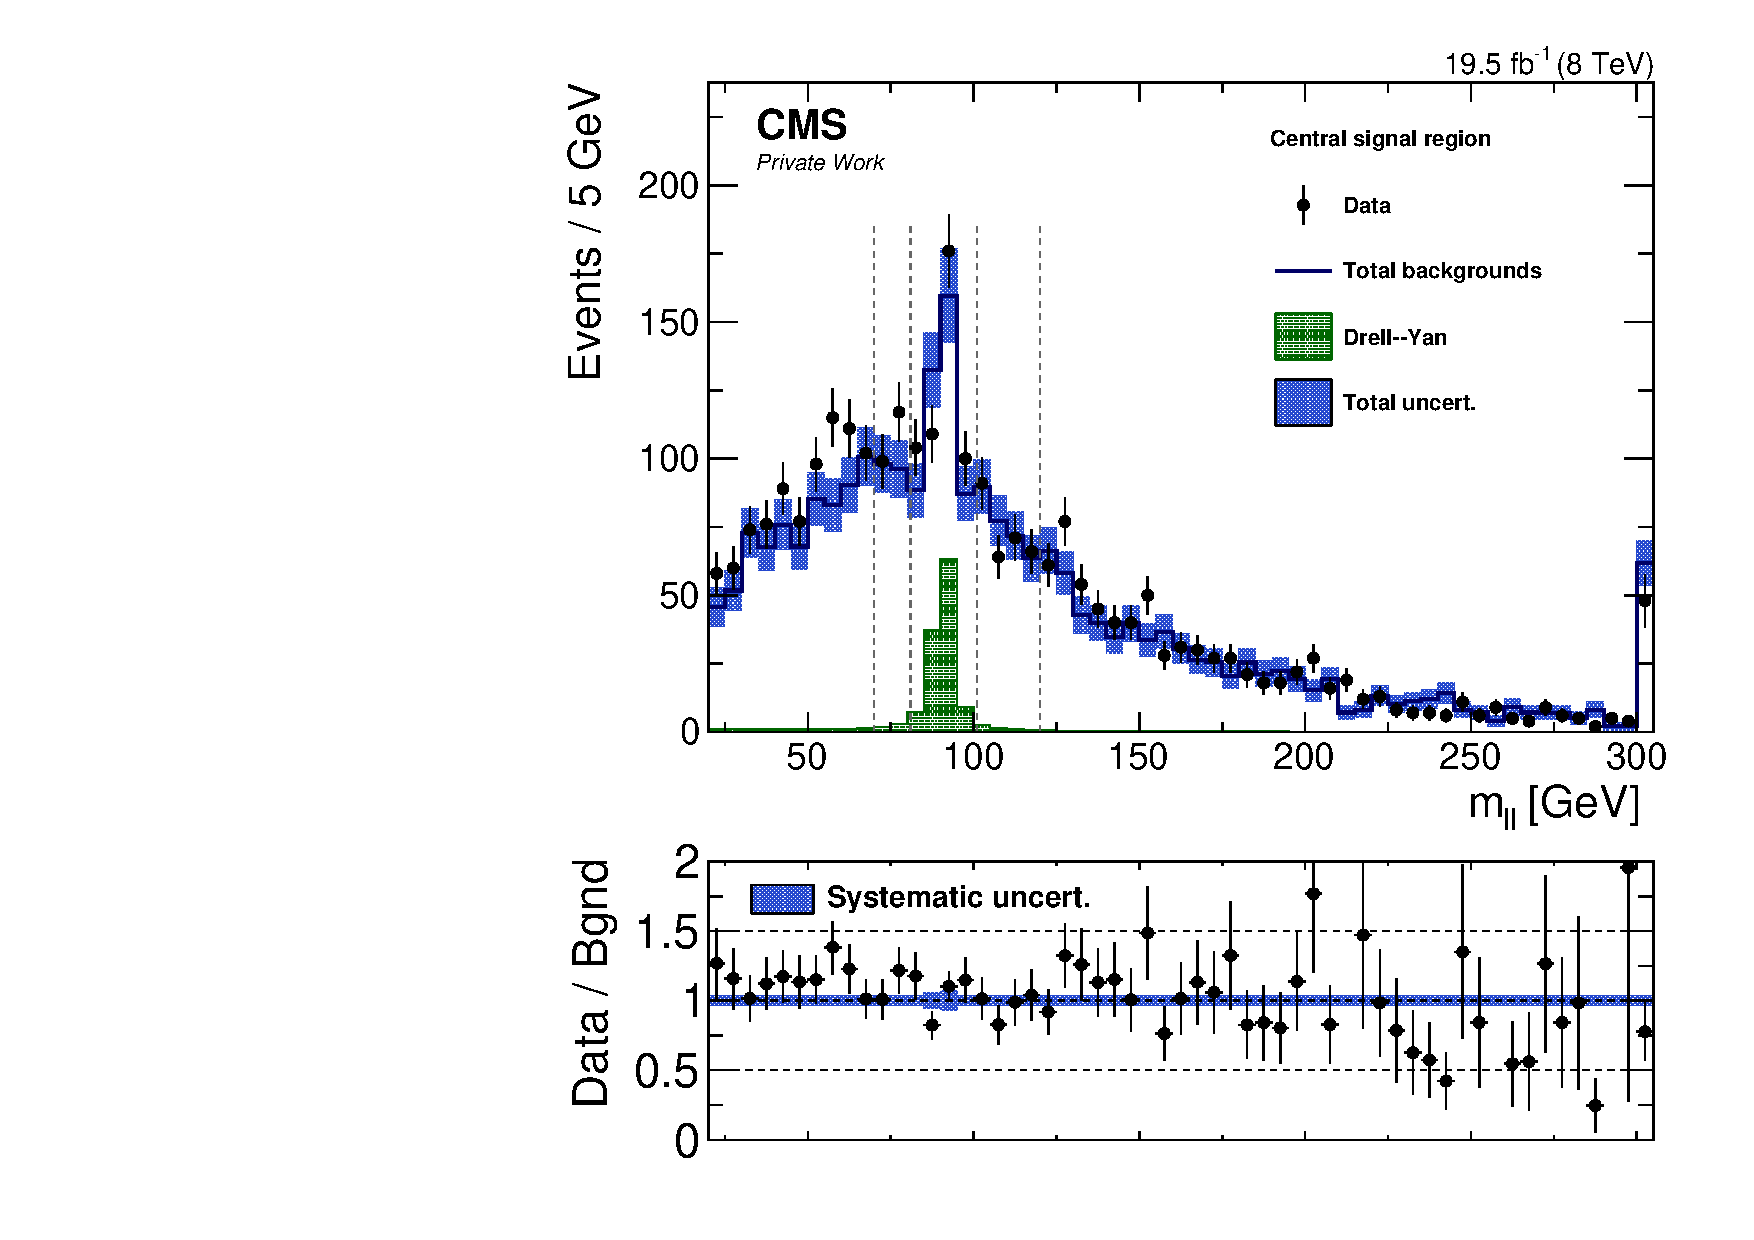
\includegraphics[width=\textwidth]{plots/results/mllResult_SignalCentral_Full2012_SF.pdf}
\end{minipage}
\begin{minipage}[t]{0.49\textwidth}
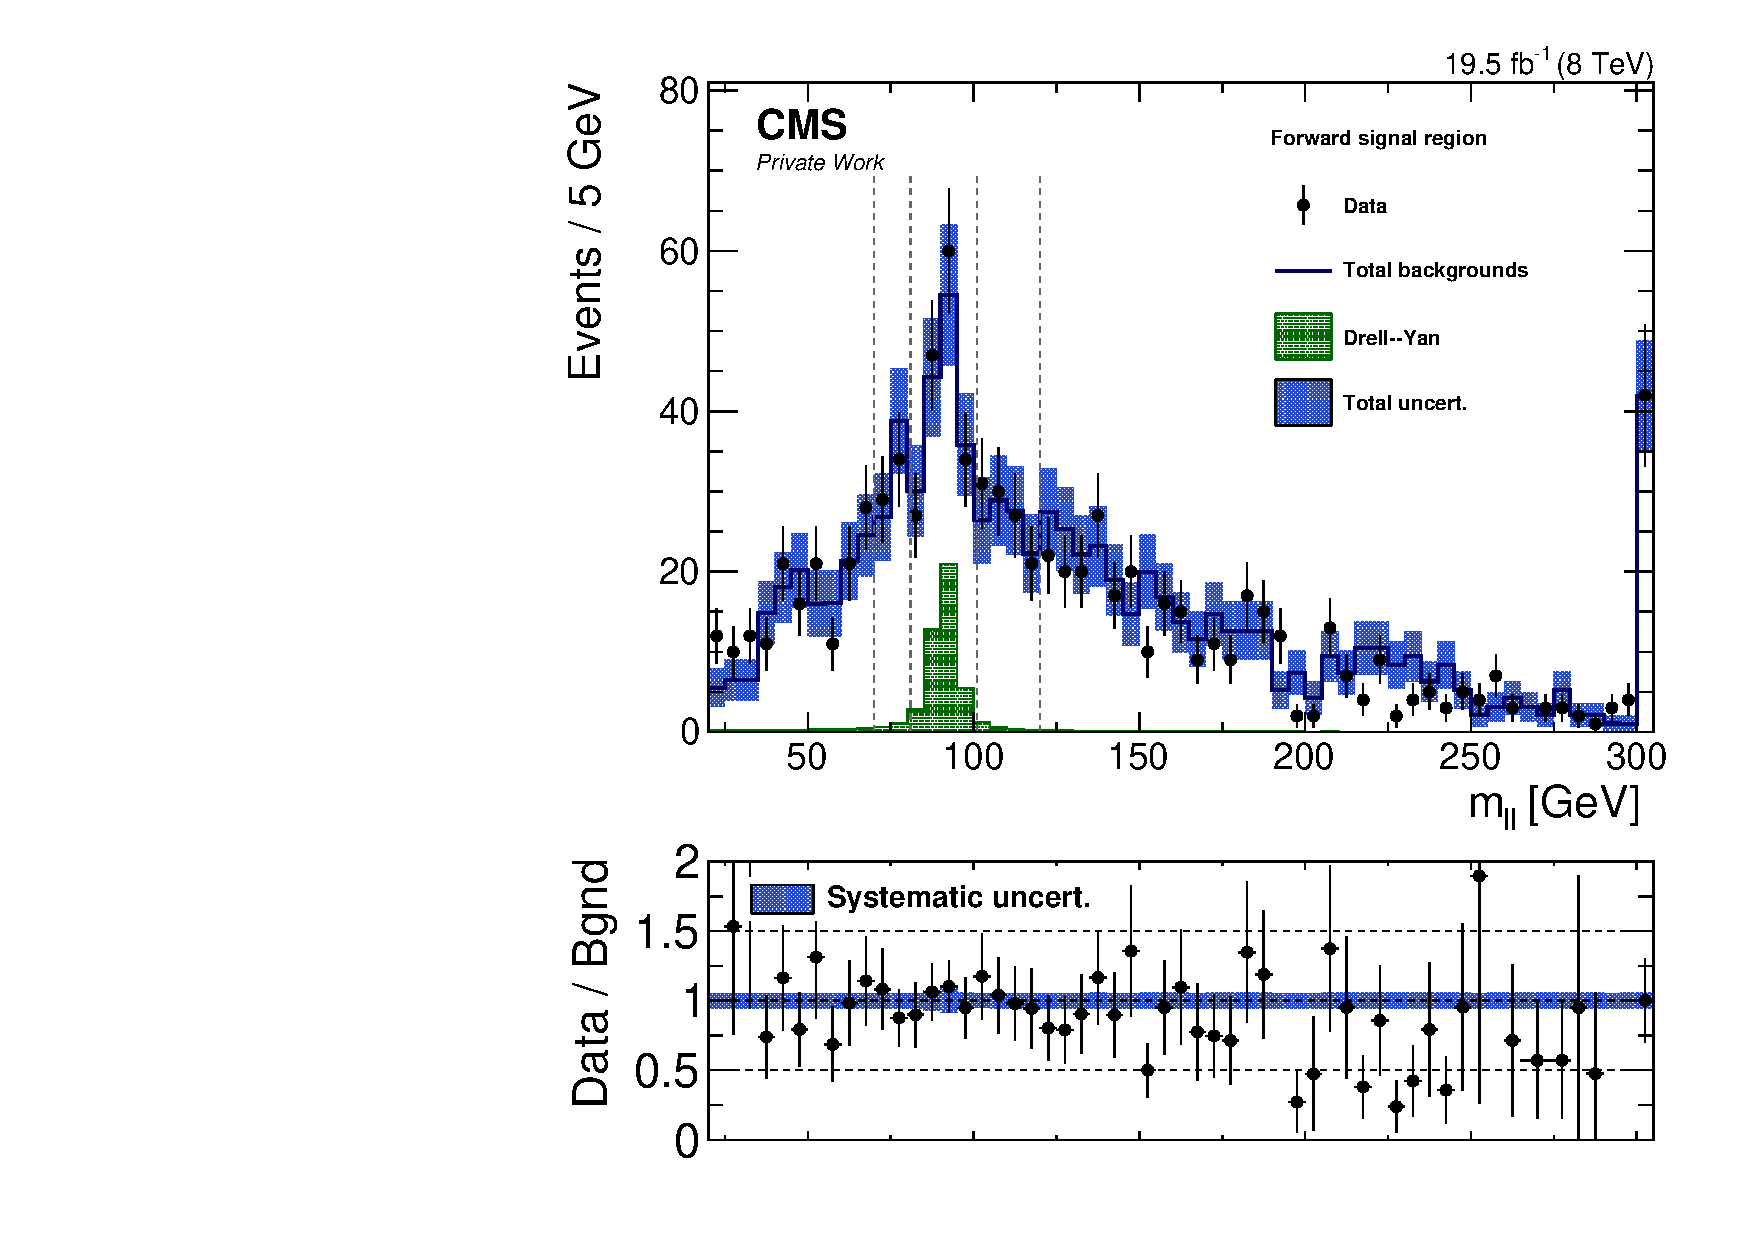
\includegraphics[width=\textwidth]{plots/results/mllResult_SignalForward_Full2012_SF.pdf}
\end{minipage}

\caption{Distribution of \mll in the signal region for the central (left) and forward (right) dilepton selection. The data is shown as black dots, while the total background prediction from data is shown as a blue histogram. The blue error bars indicate the combined statistical and systematic background uncertainty in each bin. The contribution from Drell--Yan backgrounds is shown as a green histogram. The dashed lines indicates the boundaries of the three mass bins. Beneath the plot the ratio of data to the background prediction is shown. The error bars include the statistical uncertainties of data and background, while the blue band indicates the systematic uncertainties on the background. }
\label{fig:resultsCC}
\end{figure} 


\begin{table}[btp]
 \renewcommand{\arraystretch}{1.3}
 \setlength{\belowcaptionskip}{6pt}
 \scriptsize
 \centering
 \caption{Results of the counting experiment in the six signal regions.
     The statistical and systematic uncertainties are added in quadrature, except for the flavor-symmetric backgrounds. The presented differences between the observed and estimated yields are obtained with a maximum likelihood fit (see text).    Low-mass refers to $20\GeV < \mll < 70$\GeV, on-\Z to  $81\GeV < \mll < 101$\GeV, and high-mass to $\mll > 120$\GeV.
     }
  \label{tab:METresults2012}
  \begin{tabular}{l| cc | cc | cc}

    							& \multicolumn{2}{c}{low-mass} & \multicolumn{2}{c}{on-\Z} & \multicolumn{2}{c}{high-mass} \\ 

    \hline
                                &  Central        & Forward  &  Central  & Forward   &  Central        & Forward \\ 

    \hline
        Observed       &  865                   & 154              &  494            &  176       &   849           &   381    \\

    \hline
        Flav.-sym.    & $746\pm27\pm26$        & $144\pm12\pm7$  &  $368\pm19\pm13$ & $137\pm11\pm7$ & $789\pm28\pm28$ & $411\pm20\pm21$ \\

            Drell--Yan          & $8.6\pm2.7$            & $2.6\pm0.8$      & $119\pm21$ & $43\pm9$ & $2.7\pm0.8$ & $1.2\pm0.4$ \\

    \hline
            Total est.          & $755\pm38$            & $147\pm14$      & $488\pm31$ & $180\pm16$ & $792\pm39$ & $413\pm30$ \\

    \hline
         Obs. - est.  & $109\pm48$      & $7\pm19$ & $6\pm38 $ & $-5\pm21$ & $57\pm50$ & $-32\pm37 $ \\ 

    \hline
   Significance      & 2.2~$\sigma$    &  0.4~$\sigma$  & 0.1~$\sigma$ & $<$0.1~$\sigma$ & 1.1~$\sigma$ & $<$0.1~$\sigma$ \\ 


  \end{tabular}
\end{table}



In the Tables~\ref{tab:METresults2012EE} and~\ref{tab:METresults2012MM}, the results are shown separately for \EE and \MM events. As expected from the fact that \rmue is larger than one, the yields in the \MM channel are slightly larger than in the \EE channel. For the flavour-symmetric backgrounds, and therefore also for the total background estimates and the difference of observation and estimation, the yields in the \EE and \MM channels do not exactly add up to those in the combined SF channel presented in Table~\ref{tab:METresults2012}. This is caused by the the weighted average of the two methods to determine the correction factors used to translate from OF into the different SF channels, which is calculated separately for \Rsfof, \Reeof, and \Rmmof, as discussed in Section~\ref{sec:combinedRSFOF}. Comparing the two channels, consistent results are observed between them, except for the slight excess in the high-mass central region, which is driven dominantly from \EE events. Especially for the larger excess in the low-mass central region, the observation agrees with the expected behaviour of the different flavours. The signal yields of $47\pm25$ and $67\pm29$ in the \EE and \MM channels correspond to a value of \rmue for this hypothetical signal of $1.19\pm0.41$, in good agreement with the value of $1.09\pm0.11$ measured in the Drell--Yan control region (see Section~\ref{sec:rmue}).

\begin{table}[hbtp]
 \renewcommand{\arraystretch}{1.3}
 \setlength{\belowcaptionskip}{6pt}
 \scriptsize
 \centering
 \caption{Results of the counting experiment for \EE events only.
     The statistical and systematic uncertainties are added in quadrature, except for the flavor-symmetric backgrounds. The presented differences between the observed and estimated yields are obtained with a maximum likelihood fit (see text).    Low-mass refers to $20 < \mll < 70$\GeV, on-\Z to  $81 < \mll < 101$\GeV, and high-mass to $\mll > 120$\GeV.
     }
  \label{tab:METresults2012EE}
  \begin{tabular}{l| cc | cc | cc}

    							& \multicolumn{2}{c}{low-mass} & \multicolumn{2}{c}{on-\Z} & \multicolumn{2}{c}{high-mass} \\ 

    \hline
                                &  Central        & Forward  &  Central  & Forward   &  Central        & Forward \\ 

    \hline
        Observed       &  389                   & 53              &  232            &  86       &   401           &   195    \\

    \hline
        Flav.-sym.    & $337\pm12\pm19$        & $61\pm5\pm6$  &  $166\pm8\pm9$ & $58\pm5\pm5$ & $357\pm12\pm21$ & $175\pm8\pm17$ \\

            Drell--Yan          & $4.3\pm1.3$            & $1.2\pm0.4$      & $62\pm11$ & $21\pm5$ & $1.5\pm0.5$ & $0.7\pm0.2$ \\

    \hline
            Total est.          & $342\pm23$            & $62\pm8$      & $229\pm17$ & $79\pm9$ & $358\pm24$ & $175\pm19$ \\

    \hline
         Obs. - est.  & $47\pm25$      & $-10\pm9$ & $3\pm21 $ & $6\pm12$ & $42\pm26$ & $19\pm18 $ \\ 

    \hline
   Significance      & 1.9~$\sigma$    &  $<$0.1~$\sigma$  & 0.1~$\sigma$ & 0.5~$\sigma$ & 1.7~$\sigma$ & 1.1~$\sigma$ \\ 


  \end{tabular}
\end{table}





\begin{table}[hbtp]
 \renewcommand{\arraystretch}{1.3}
 \setlength{\belowcaptionskip}{6pt}
 \scriptsize
 \centering
 \caption{Results of the counting experiment for \MM events only.
     The statistical and systematic uncertainties are added in quadrature, except for the flavor-symmetric backgrounds.
     Low-mass refers to $20 < \mll < 70$\GeV, on-\Z to  $81 < \mll < 101$\GeV and high-mass to $\mll > 120$\GeV.
     }
  \label{tab:METresults2012MM}
  \begin{tabular}{l| cc | cc | cc}

    							& \multicolumn{2}{c}{low-mass} & \multicolumn{2}{c}{on-\Z} & \multicolumn{2}{c}{high-mass} \\ 

    \hline
                                &  Central        & Forward  &  Central  & Forward   &  Central        & Forward \\ 

    \hline
        Observed       &  476                   & 101              &  262            &  90       &   448           &   186    \\

    \hline
        Flavor-symmetric    & $405\pm14\pm21$        & $79\pm6\pm6$  &  $200\pm10\pm10$ & $74\pm6\pm6$ & $428\pm15\pm23$ & $224\pm11\pm19$ \\

            Drell--Yan          & $4.4\pm1.4$            & $1.6\pm0.6$      & $58\pm10$ & $25\pm6$ & $1.2\pm0.4$ & $0.7\pm0.2$ \\

    \hline
            Total estimated          & $409\pm26$            & $80\pm9$      & $258\pm18$ & $100\pm11$ & $429\pm27$ & $225\pm22$ \\

    \hline
         Observed - estimated  & $67^{+29}_{-29}$      & $20^{+13}_{-13}$ & $3^{+22}_{-23} $ & $-11^{+13}_{-13}$ & $19^{+29}_{-29}$ & $-40^{+21}_{-21} $ \\ 

    \hline
   Significance      & 2.3~$\sigma$    &  1.6~$\sigma$  & 0.2~$\sigma$ & $<$0.1~$\sigma$ & 0.6~$\sigma$ & $<$0.1~$\sigma$ \\ 


  \end{tabular}
\end{table}





\subsection*{Investigating the low-mass central region}
While a significance of $2.2\sigma$ is no clear indication for the presence of new physics, more detailed studies into the properties of this excess are conducted. 

The development of the excess during the data taking period in 2012 is shown on the left side of Figure~\ref{fig:timeDependece}, while the right side shows the low-mass forward region for comparison. The data sample is split into 10 bins, each corresponding to 2\,$fb^{-1}$ within 1\%, except for the last which corresponds to only  about 1.5\,$fb^{-1}$. For each of these bins the observed SF yield and the prediction for flavour-symmetric backgrounds from OF is shown, together with the difference of the two. The very small contribution from Drell--Yan backgrounds of typically less than 1 event per bin is neglected in this representation of the result. For the first four bins, corresponding to the first 8\,$fb^{-1}$ of data collected in 2012, the SF yield is significantly higher than the prediction from OF. This effect diminishes in the fifth bin, where the SF yield decreases and the prediction from OF increases. In the following five bins, representing the second half of the data sample, good agreement is observed between the observed SF yield and the prediction from OF. This change in behaviour between the two halves is caused in roughly equal manner by a decrease in the observed SF yield and an increase in the observed OF yield per bin. In contrast to this observations, the SF yield and the background prediction are compatible within uncertainties for all bins in the low-mass forward region. The difference between the two therefore fluctuates around zero.

\begin{figure}[htbp]
\centering
\begin{minipage}[t]{0.49\textwidth}
  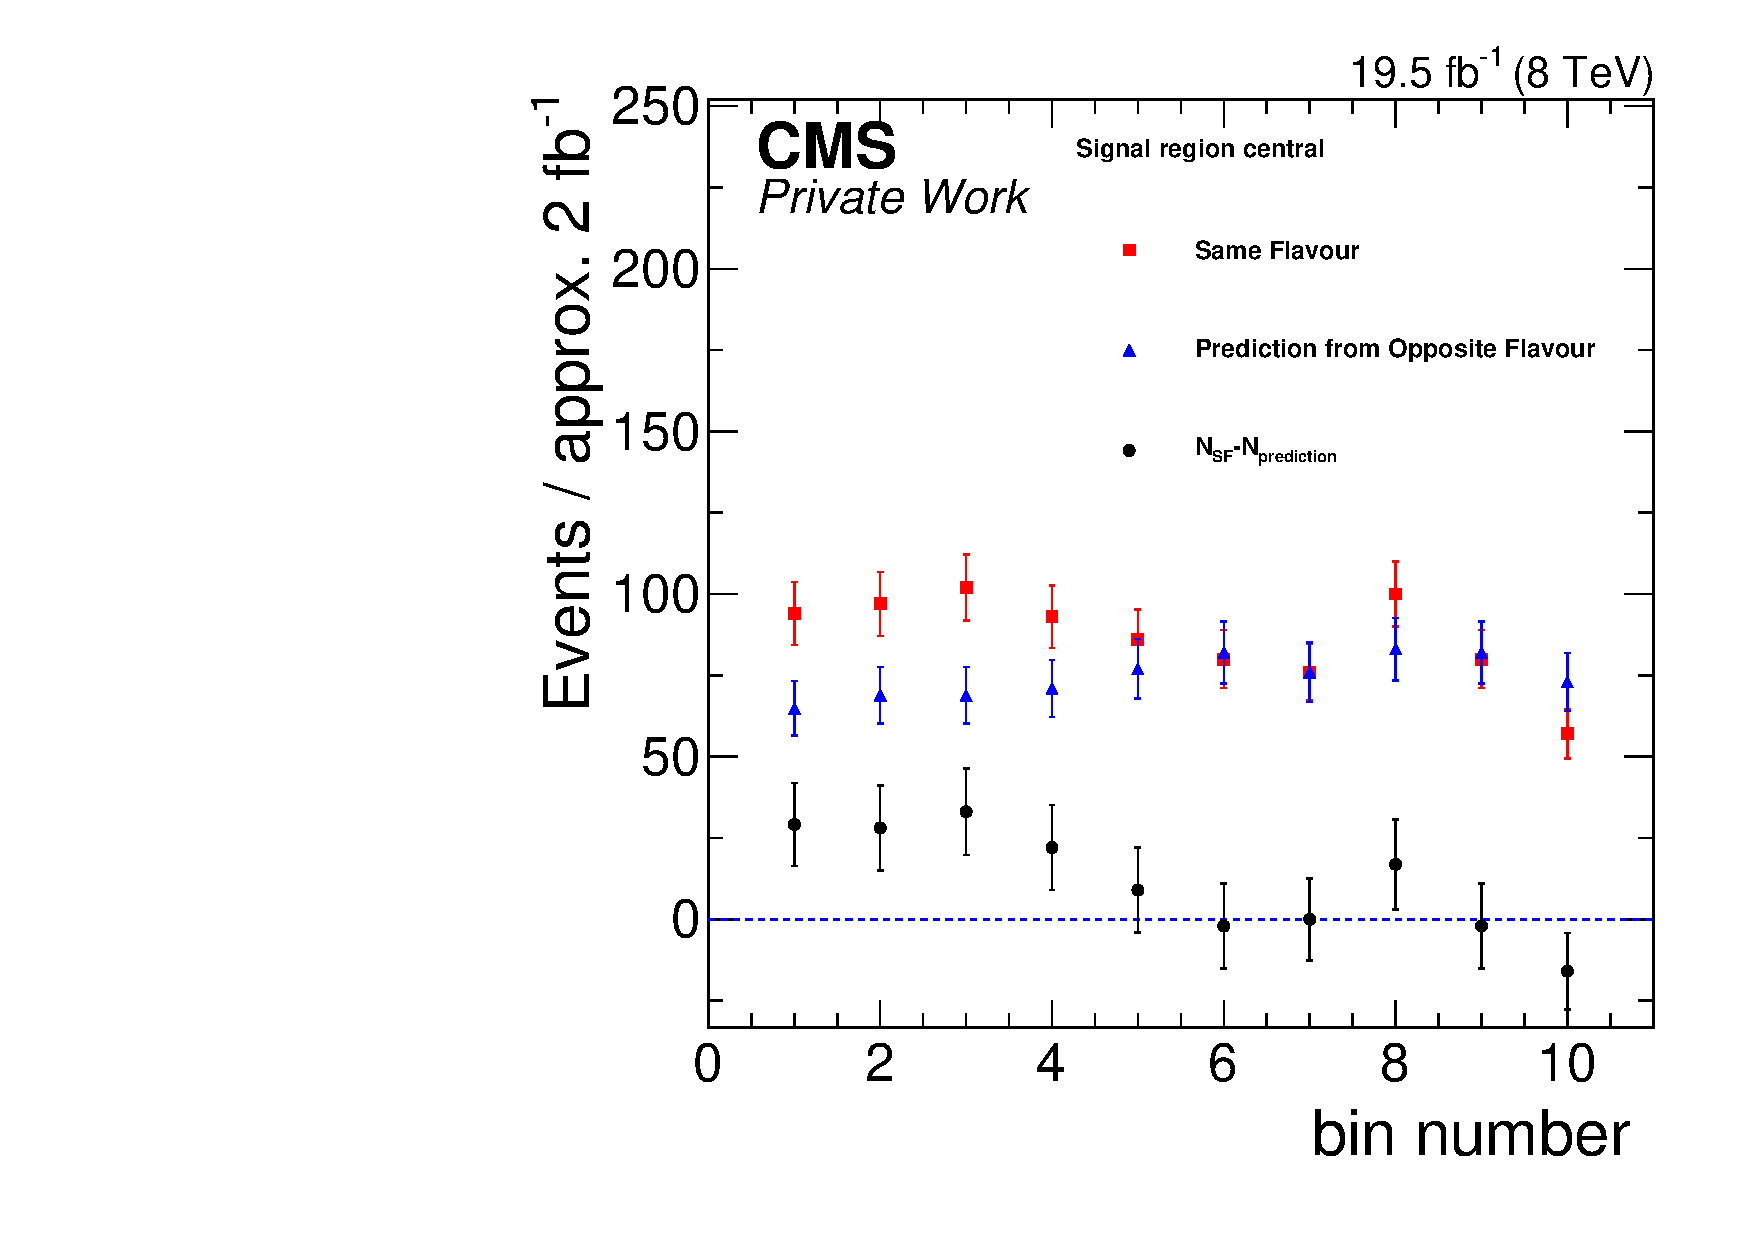
\includegraphics[width=\textwidth]{plots/results/YieldvsLumi_Bins_SignalCentral_Mll_edgeMassFull2012.pdf}
\end{minipage}
\begin{minipage}[t]{0.49\textwidth}
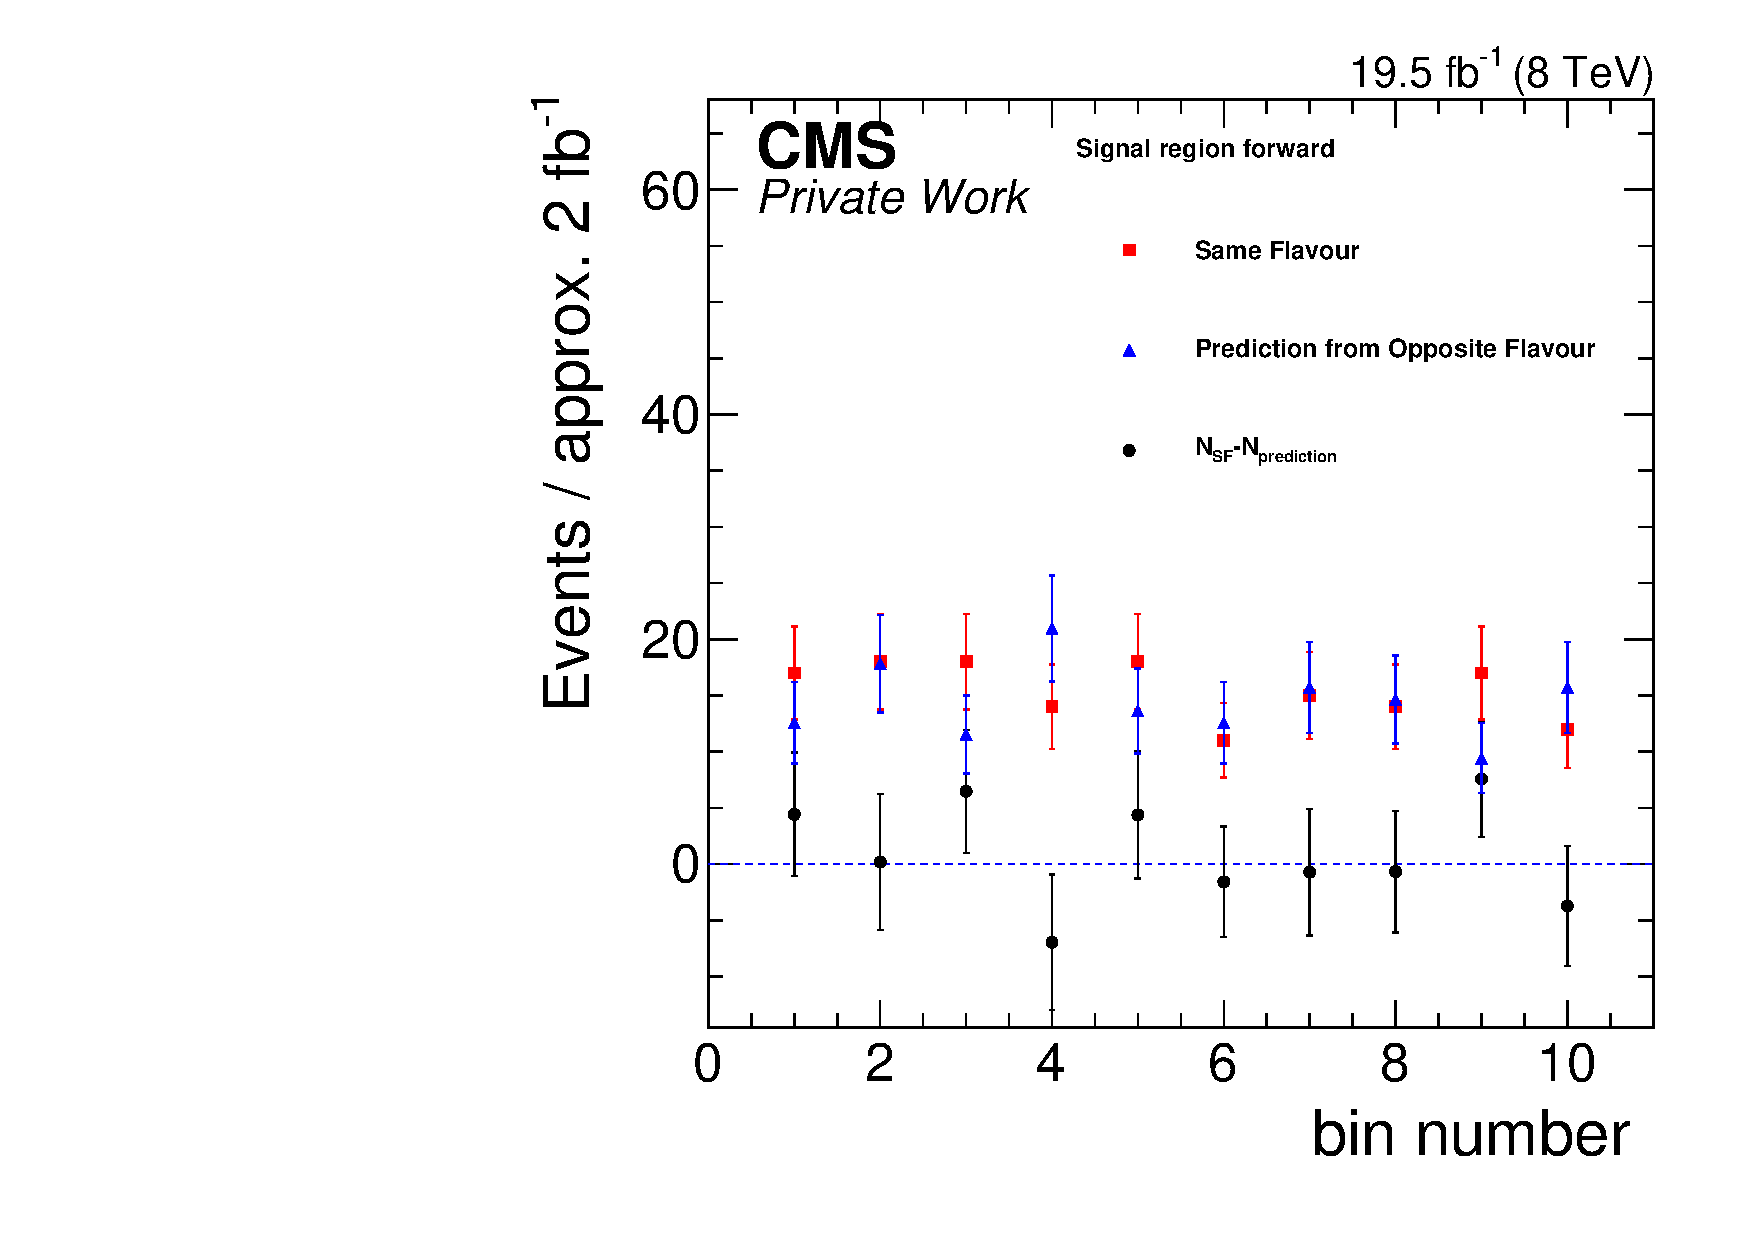
\includegraphics[width=\textwidth]{plots/results/YieldvsLumi_Bins_SignalForward_Mll_edgeMassFull2012.pdf}
\end{minipage}

\caption{Observed SF yields and background prediction from OF as well as the difference of these two in the low-mass central (left) and forward (right) signal region in 10 bins of roughly equal integrated luminosity. Non-flavour-symmetric backgrounds are not included in this representation of the result.}
\label{fig:timeDependece}
\end{figure}

To get a clearer picture of the properties of the excess and also to check for some of the more obvious possible systematic effects that might cause it, the counting experiment in the low-mass central region is repeated several times, varying the selection requirements. The results are shown in Table~\ref{tab:CountingCrosschecks}. As no Drell-Yan prediction for the on-\Z region is available for the different configurations, the observed yield is extrapolated into the low-mass region after subtraction of flavour-symmetric background using the prediction from OF. For all these cross-checks presented here one has to keep in mind that for the background prediction from OF the \Rsfof factor derived for the default selection is used.

As the signal region is dominated by events containing b-tagged jets, it seems natural to test the excess for its b-tag content. Splitting the data sample into events with at least one and those without a b-tag, it is evident that, while constituting about 23\% of the total yield, less than 10\% of the excess is located in events without a b-tagged jet. 

In addition to the default selection of $\pt > \unit{20}{\giga\electronvolt}$, four other configurations for the lepton \pt requirement are tested. Three of them feature asymmetric cuts on the \pt of the leading and trailing lepton. The selection of $\pt > 20(10)$ and $ \pt > 30(10)\GeV$ extend the acceptance of the analysis to lower trailing lepton \pt. For both of these selections, an increased signal yield is observed. On the other hand, raising the trailing \pt threshold to 30\GeV disproportionally reduces the observed excess, retaining only about 13\% of the excess yield compared to 23\% of the overall event yield. 

Although it has already been established in Section~\ref{sec:validation} that non-prompt leptons only account for a small part of the selected data sample and are also fully flavour-symmetric, the counting experiment is repeated with significantly tighter isolation requirements. The relative isolation is required to be smaller than 5\%, reducing the size of the selected sample by about one third. The number of observed signal events is reduced by almost exactly the same amount. This further increases the confidence that the observed effect is due to prompt lepton production.

To test for a possible pileup dependence of the observed effect, the sample is split into three subsets of similar size depending on the number of reconstructed vertices. The events are categorised as either low-pileup ($N_{\mathrm{vtx}} < $13), mid-pileup (13 $\leq N_{\mathrm{vtx}} <$ 17) or high-pileup ($N_{\mathrm{vtx}} \geq $17). The excess is observed consistently in all three subsets, excluding a possible pileup dependence of excess. 

Three additional \MET reconstructions are tested. TC \MET and type-I corrected PF \MET have been described in Section~\ref{sec:PF}. In addition to these general algorithms, an analysis-specific definition of missing $H_{\mathrm{T}}$ is used, which is calculated using only selected jets and leptons. It is defined as the absolute value of the negative vector sum of the the transverse momenta of these objects: 
\begin{equation*}
H_{\mathrm{T}}^{\mathrm{miss}} = | -(\sum\limits_{\mathrm{jets}}\vec{p}_{\mathrm{T}} + \sum\limits_{\mathrm{leptons}}\vec{p}_{\mathrm{T}}) |.
\end{equation*}
The signal region requirements of $\unit{100}{\giga\electronvolt}$ and $\unit{150}{\giga\electronvolt}$, depending on \njets, are applied for each of these \MET values.  Both the use of type-I corrected PF \MET and missing $H_{\mathrm{T}}$ lead to higher event yields in the signal region. Judging by the size of the Drell--Yan background, TC \MET and $H_{\mathrm{T}}^{\mathrm{miss}}$ have significantly worse \MET resolution compared to both types of PF \MET. The excess is present in all three cases and is therefore not likely to be caused by a faulty \MET reconstruction. 

Separating the data sample into events with low \HT ($\unit{100}{\giga\electronvolt} < \HT <\unit{300}{\giga\electronvolt}$) and high \HT ($\HT > \unit{300}{\giga\electronvolt}$) creates two subsets of roughly the same size. The excess is present in both subsets with similar strength. 
 


\begin{table}[hbtp]
 \renewcommand{\arraystretch}{1.3}
 \setlength{\belowcaptionskip}{6pt}
 \centering
 \caption{Results of the counting experiment in the low-mass central signal region for different variations of the event selection. The observed event yield in SF events is compared with the combined estimate from flavour-symmetric and Drell--Yan backgrounds. The estimate for the Drell--Yan backgrounds is obtained by extrapolating the event yield in the on-Z signal region after subtraction of flavour-symmetric backgrounds to the low-mass region using the \Routin factor.}
  \label{tab:CountingCrosschecks}
  \begin{tabular}{l|c|c|c|c}
                                &  SF        & Flavour-symmetric  &  Drell--Yan  & Observed - Estimates \\ 

    \hline
    \hline
 & \multicolumn{4}{c}{b-tagging}\\ 
\hline 
        no b-tags       &  202                   & 188.5$\pm$15.4              &  7.1$\pm$2.5            &  6.3$\pm$21.1 \\
        $\geq$ 1 b-tags       &  663                   & 558.4$\pm$31.0              &  1.9$\pm$0.7            &  102.7$\pm$40.3 \\
\hline 
 & \multicolumn{4}{c}{lepton \pt requirement} \\ 
\hline 
        \pt > 20(10)\GeV       &  1474                   & 1290.2$\pm$58.6              &  11.4$\pm$4.1            &  172.5$\pm$70.1 \\
        \pt > 30(10)\GeV       &  1262                   & 1114.8$\pm$52.1              &  11.3$\pm$4.1            &  135.9$\pm$63.2 \\
        \pt > 30(20)\GeV       &  761                   & 674.0$\pm$35.5              &  9.0$\pm$3.3            &  78.0$\pm$45.1 \\
        \pt > 30\GeV       &  296                   & 275.7$\pm$19.4              &  6.5$\pm$2.3            &  13.8$\pm$26.0 \\
\hline 
 & \multicolumn{4}{c}{tight lepton isolation} \\ 
\hline 
        rel. isolation < 0.05       &  572                   & 491.5$\pm$28.4              &  7.1$\pm$2.6            &  73.3$\pm$37.2 \\
\hline 
 & \multicolumn{4}{c}{pileup} \\ 
\hline 
        $N_{\text{vtx}} <$ 13       &  332                   & 289.9$\pm$20.0              &  3.3$\pm$1.2            &  38.8$\pm$27.1 \\
        13 $\leq N_{\text{vtx}}$ < 17       &  242                   & 212.8$\pm$16.5              &  0.9$\pm$0.3            &  28.3$\pm$22.7 \\
        $N_{\text{vtx}} \geq$ 17       &  291                   & 244.2$\pm$18.0              &  4.8$\pm$1.7            &  41.9$\pm$24.8 \\
\hline 
 & \multicolumn{4}{c}{\MET reconstructions}\\
\hline 
        type I corrected PF \MET       &  1034                   & 923.3$\pm$45.0              &  9.4$\pm$3.4            &  101.3$\pm$55.4 \\
        track corrected \MET       &  850                   & 702.3$\pm$36.6              &  26.3$\pm$9.4            &  121.3$\pm$47.7 \\
        missing $H_{\mathrm{T}}$       &  1171                   & 942.5$\pm$45.7              &  50.8$\pm$18.1            &  177.6$\pm$59.9 \\
\hline 
 & \multicolumn{4}{c}{$H_{\mathrm{T}}$}\\
\hline 
        100\GeV $< H_{\mathrm{T}} < $ 300\GeV        &  455                   & 401.3$\pm$24.7              &  1.4$\pm$0.5            &  52.3$\pm$32.7 \\
        $H_{\mathrm{T}} > $ 300\GeV        &  410                   & 344.6$\pm$22.4              &  7.5$\pm$2.7            &  57.9$\pm$30.3 \\
\hline 


  \end{tabular}
\end{table}




The distributions of several observables in the low-mass signal region is shown in Figure~\ref{fig:dependencies}. Each time the observed data is compared to the prediction from OF events. The contribution from Drell--Yan backgrounds is neglected. The excess is located predominantly in events with one or two b-tagged jets, but no excess is observed for higher b-tag multiplicities. Furthermore, it is located almost inclusively in events with three jets. It is present in events with a \pt of the leading lepton of up to $\unit{60}{\giga\electronvolt}$. For events with a trailing lepton \pt above $\unit{25}{\giga\electronvolt}$, only a small deviation from the expectation is observed. The excess seems to favour low values of \MET and is roughly uniformly distributed in \HT. 

In all performed studies, no evidence for systematic effects causing the observed excess is found. The two major distinguishing features of the events causing the deviation are the presence of at least one b-tagged jet and trailing leptons with very low \pt. In general, no features distinguishing the events in the excess from the dominant \ttbar background are observed in any of the performed studies. 

\begin{figure}[htbp]
\centering
\begin{minipage}[t]{0.49\textwidth}
  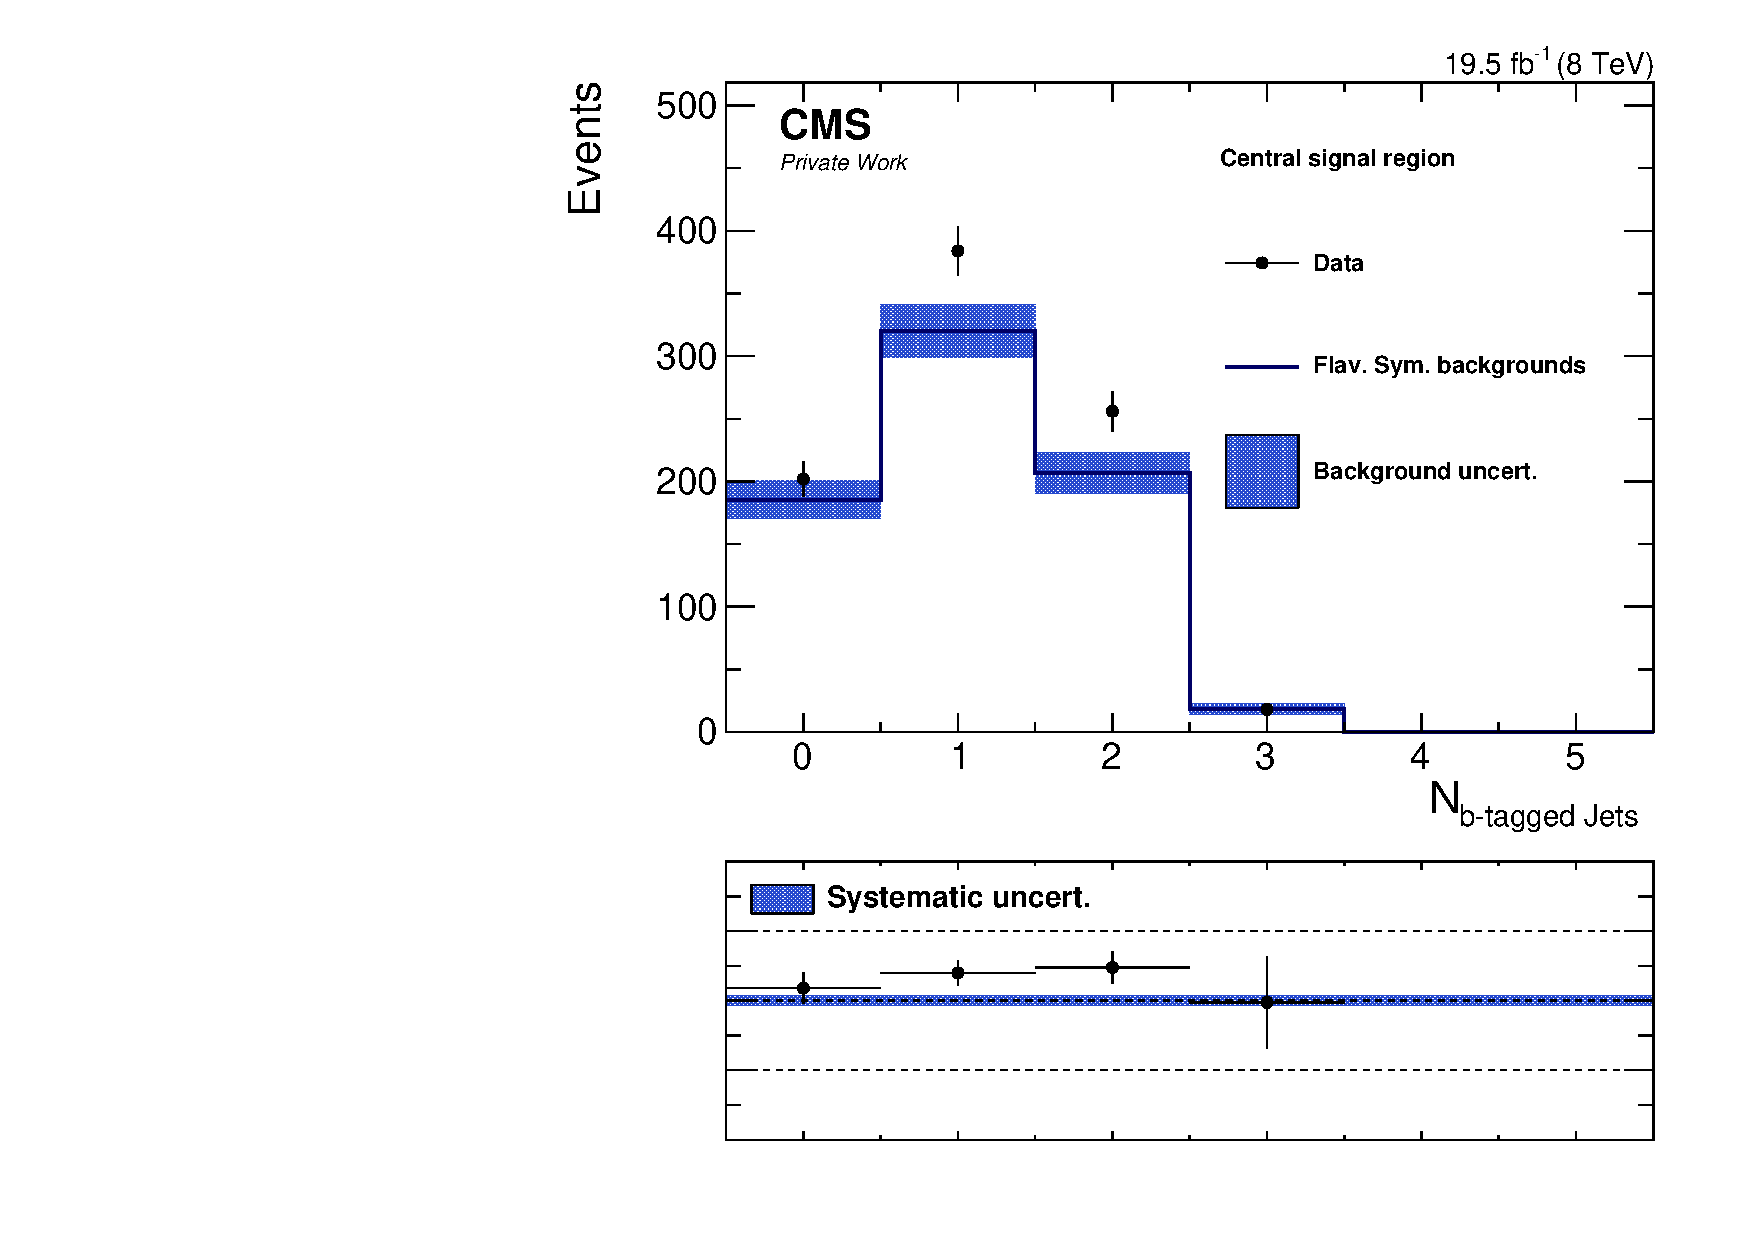
\includegraphics[width=\textwidth]{plots/results/rSFOFDependencies/rSFOFDependency_SignalCentral_NBJets_Full2012_SF_lowMass.pdf}
\end{minipage}
\begin{minipage}[t]{0.49\textwidth}
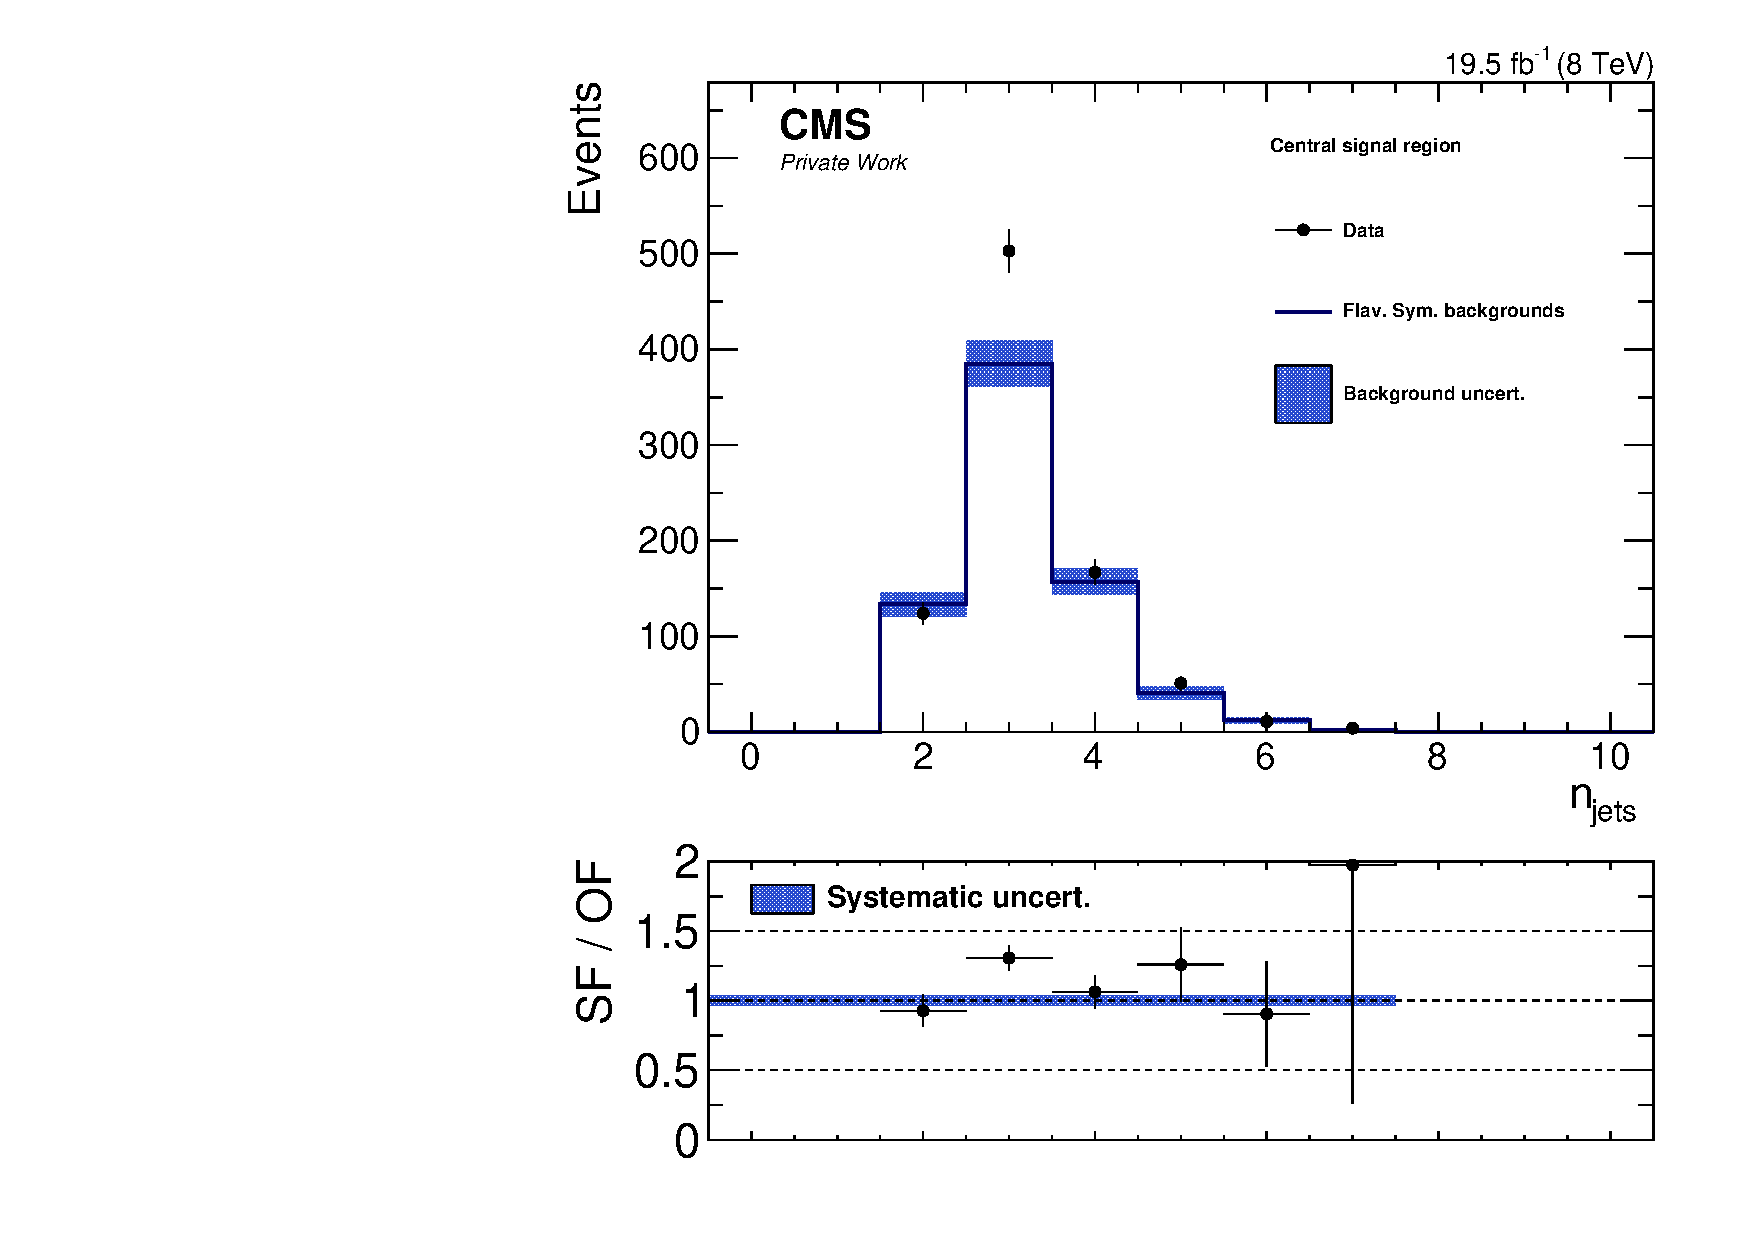
\includegraphics[width=\textwidth]{plots/results/rSFOFDependencies/rSFOFDependency_SignalCentral_NJets_Full2012_SF_lowMass.pdf}
\end{minipage}
\begin{minipage}[t]{0.49\textwidth}
  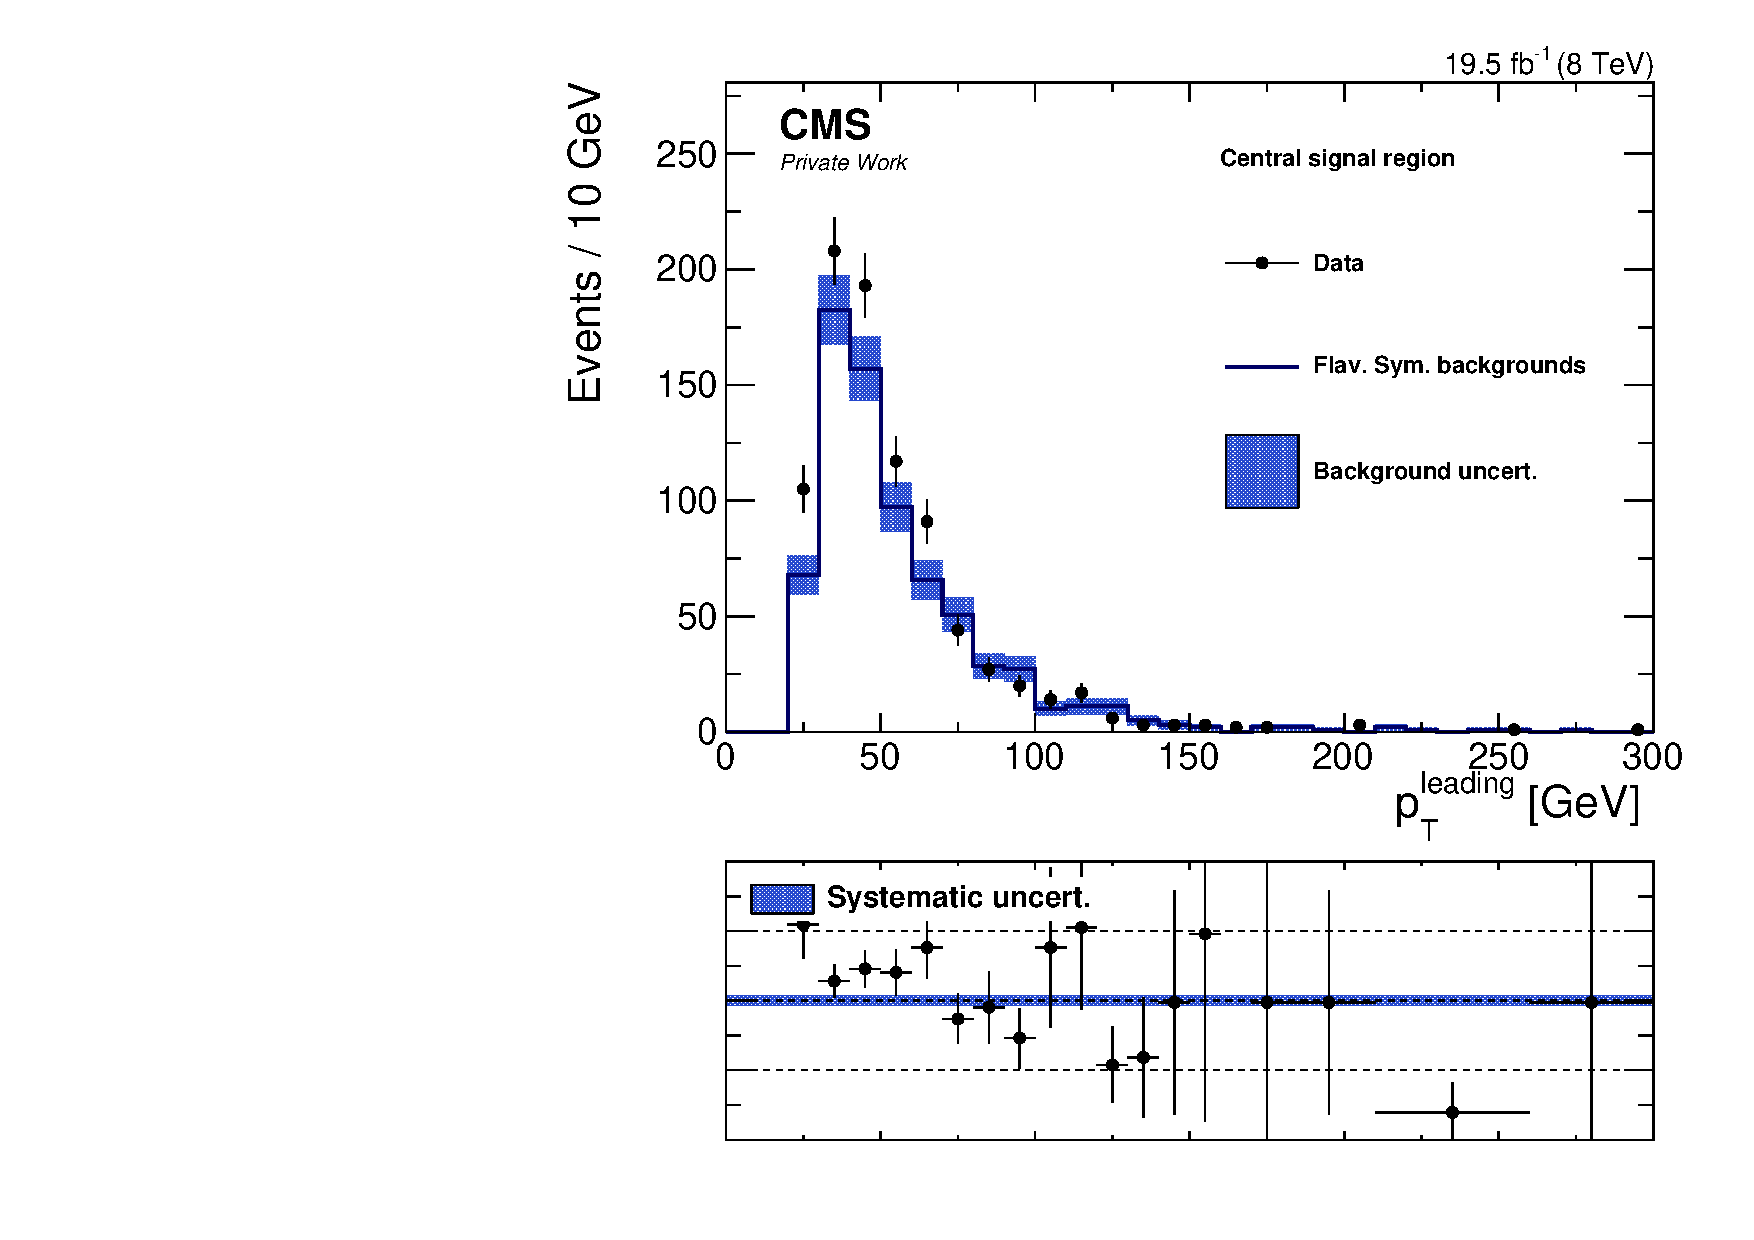
\includegraphics[width=\textwidth]{plots/results/rSFOFDependencies/rSFOFDependency_SignalCentral_LeadingPt_Full2012_SF_lowMass.pdf}
\end{minipage}
\begin{minipage}[t]{0.49\textwidth}
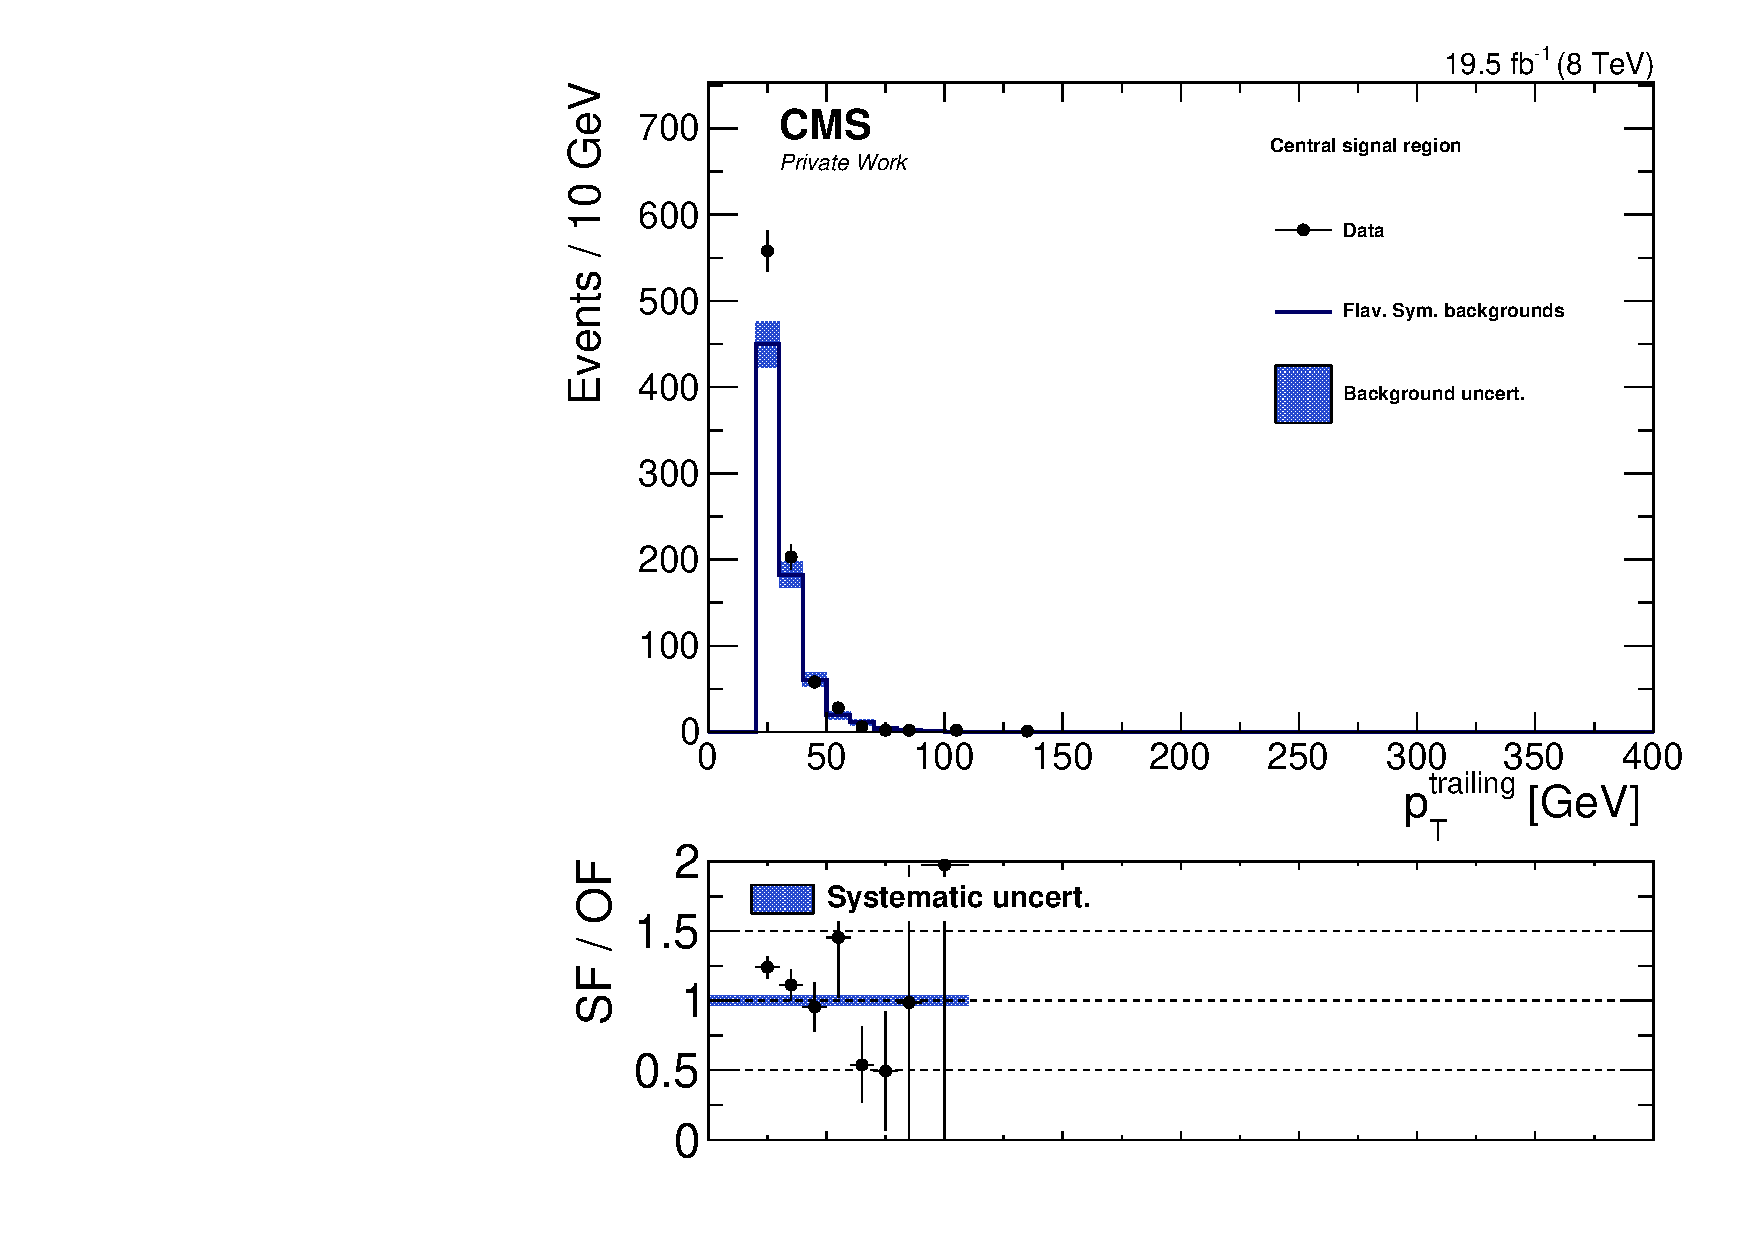
\includegraphics[width=\textwidth]{plots/results/rSFOFDependencies/rSFOFDependency_SignalCentral_TrailingPt_Full2012_SF_lowMass.pdf}
\end{minipage}
\begin{minipage}[t]{0.49\textwidth}
  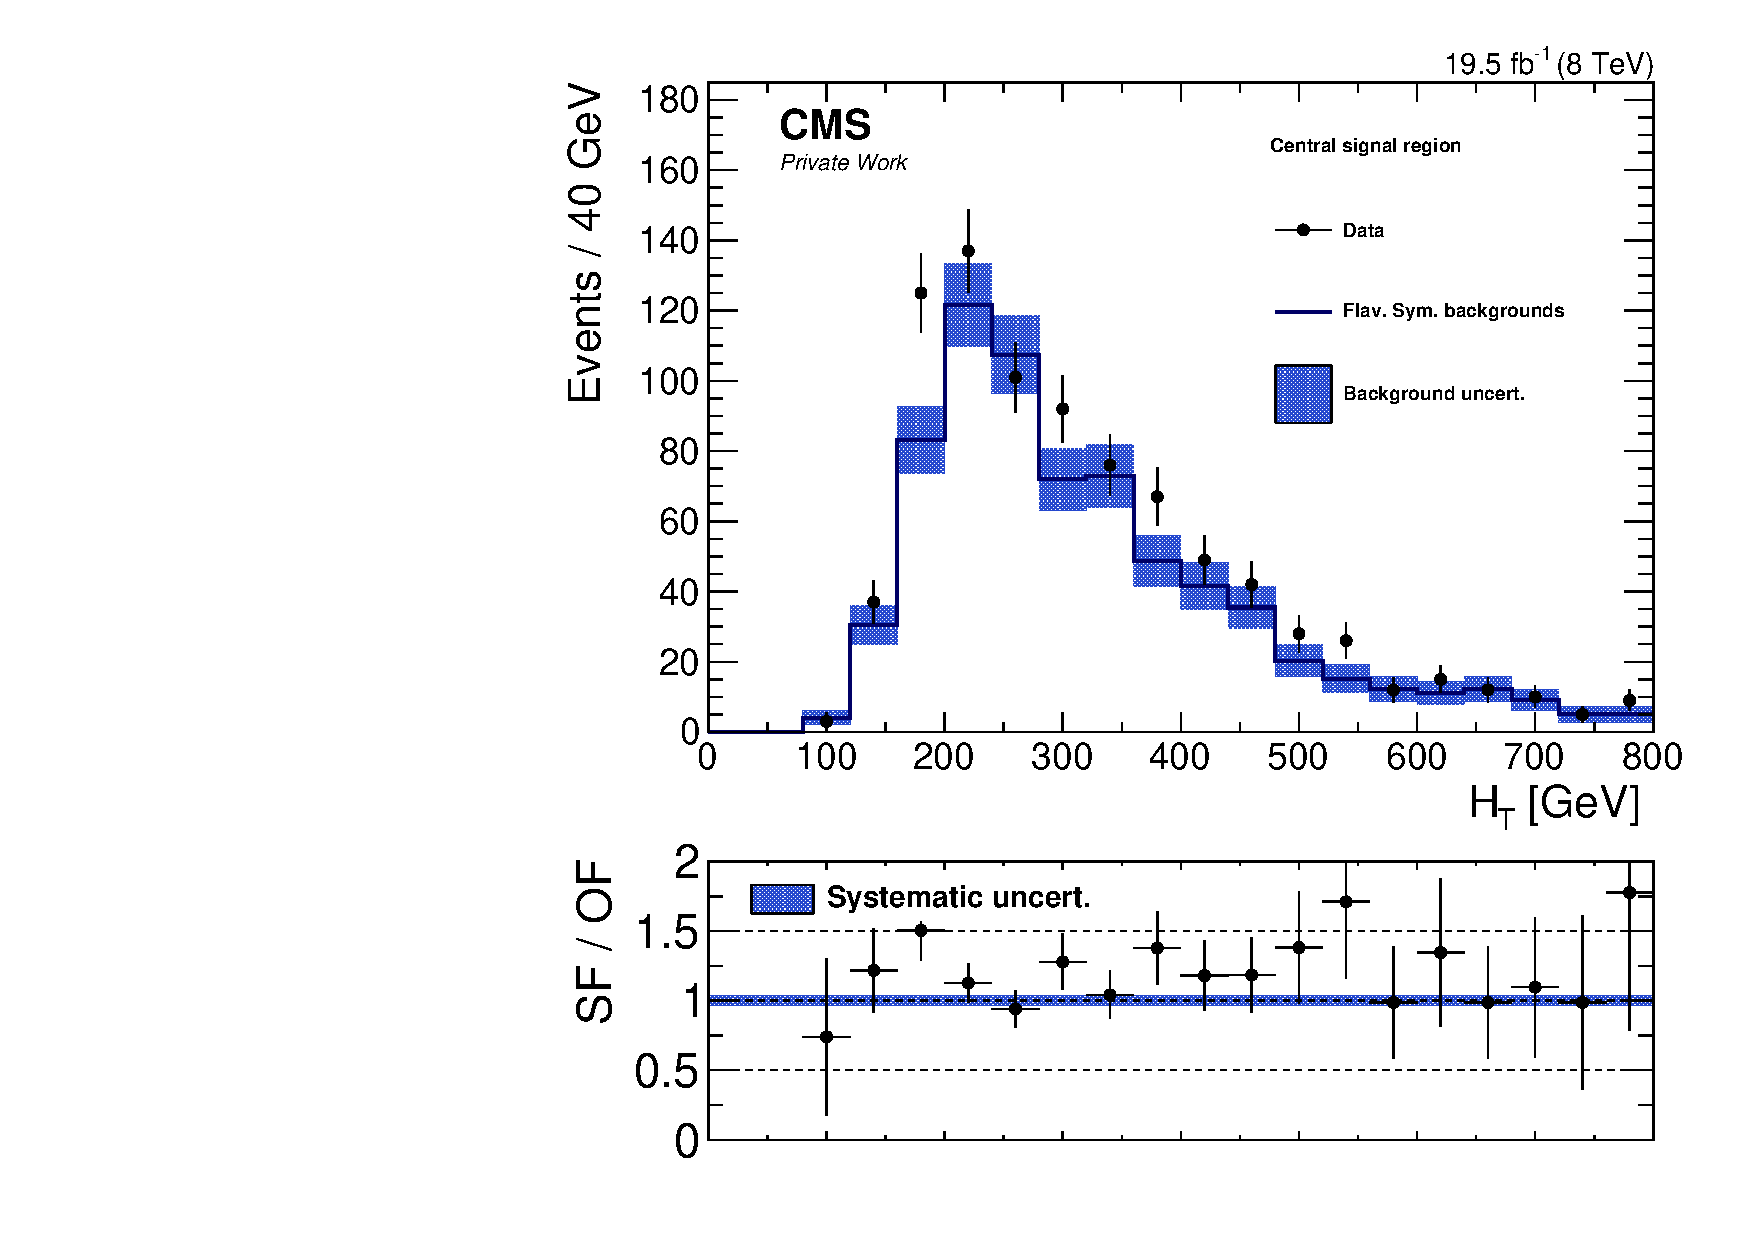
\includegraphics[width=\textwidth]{plots/results/rSFOFDependencies/rSFOFDependency_SignalCentral_HT_Full2012_SF_lowMass.pdf}
\end{minipage}
\begin{minipage}[t]{0.49\textwidth}
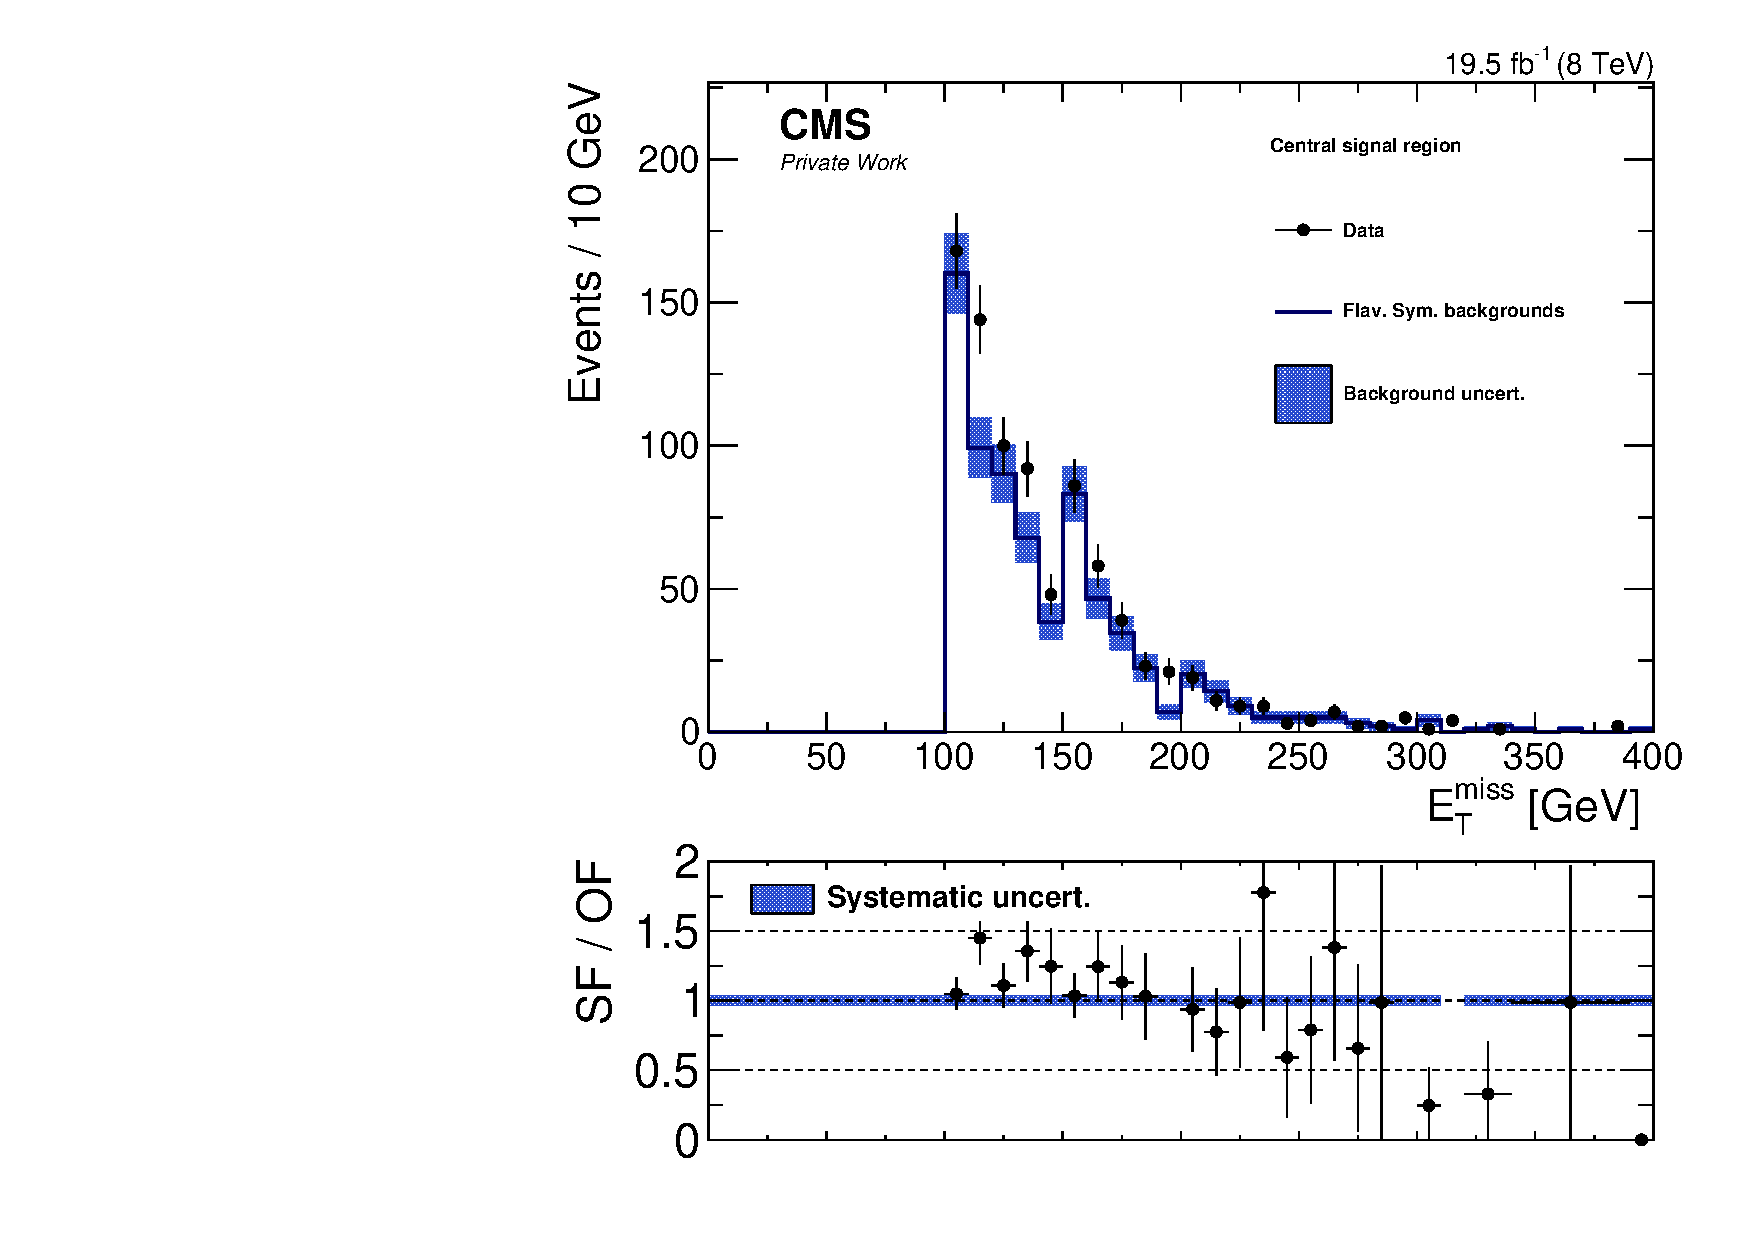
\includegraphics[width=\textwidth]{plots/results/rSFOFDependencies/rSFOFDependency_SignalCentral_MET_Full2012_SF_lowMass.pdf}
\end{minipage}
\caption{Distribution of the number of b-tagged jets (top left), jets (top right), \pt of the leading (middle left) and trailing (middle right) lepton, \HT (bottom left), and \MET (bottom right) in the low-mass central signal region. The data is shown as black dots, while the total background prediction from data is shown as a blue histogram. The blue error bars indicate the combined statistical and systematic background uncertainty in each bin. The contribution from Drell--Yan backgrounds is neglected.}
\label{fig:dependencies}
\end{figure}


\section{Interpretation in simplified models}
The absence of a clear indication for the existence of SUSY in the results of the counting experiment presented in Section~\ref{sec:candcresults} constrains the validity of supersymmetric models. To quantify the impact these results have on the allowed parameter space, they are interpreted in specific signal scenarios. Here, the two simplified models discussed in Section~\ref{sec:models} are used. 

\subsubsection{Selection efficiencies}
The impact of branching fractions, detector acceptance, and selection efficiencies on the different signal points is shown in Figure~\ref{fig:sigEff} for the example of the central signal region for the fixed-edge (left) and slepton-edge (right) models. Because of the much larger branching fraction into lepton pairs in the case of the slepton-edge model, caused by the presence of the slepton in decay chain, the overall acceptance$\times$efficiency is an order of magnitude larger in this case. As the event kinematics vary depending on the sparticle masses, the efficiency strongly depends on the position of the signal point in the $m_{\sbottom}$-$m_{\secondchi}$ plane. In general, the efficiency is low along the diagonal, where little energy is available for the decay products. Another notable feature is a decrease in efficiency around \secondchi masses of about $\unit{225}{\giga\electronvolt}$ in the case of the slepton-edge model. This is caused by the gaps in the signal acceptance between the three invariant mass regions of the counting experiment. No such effect is visible for the fixed-edge case because the signal is concentrated in the low-mass region in this model.  
\begin{figure}[htbp]
\centering
\begin{minipage}[t]{0.49\textwidth}
  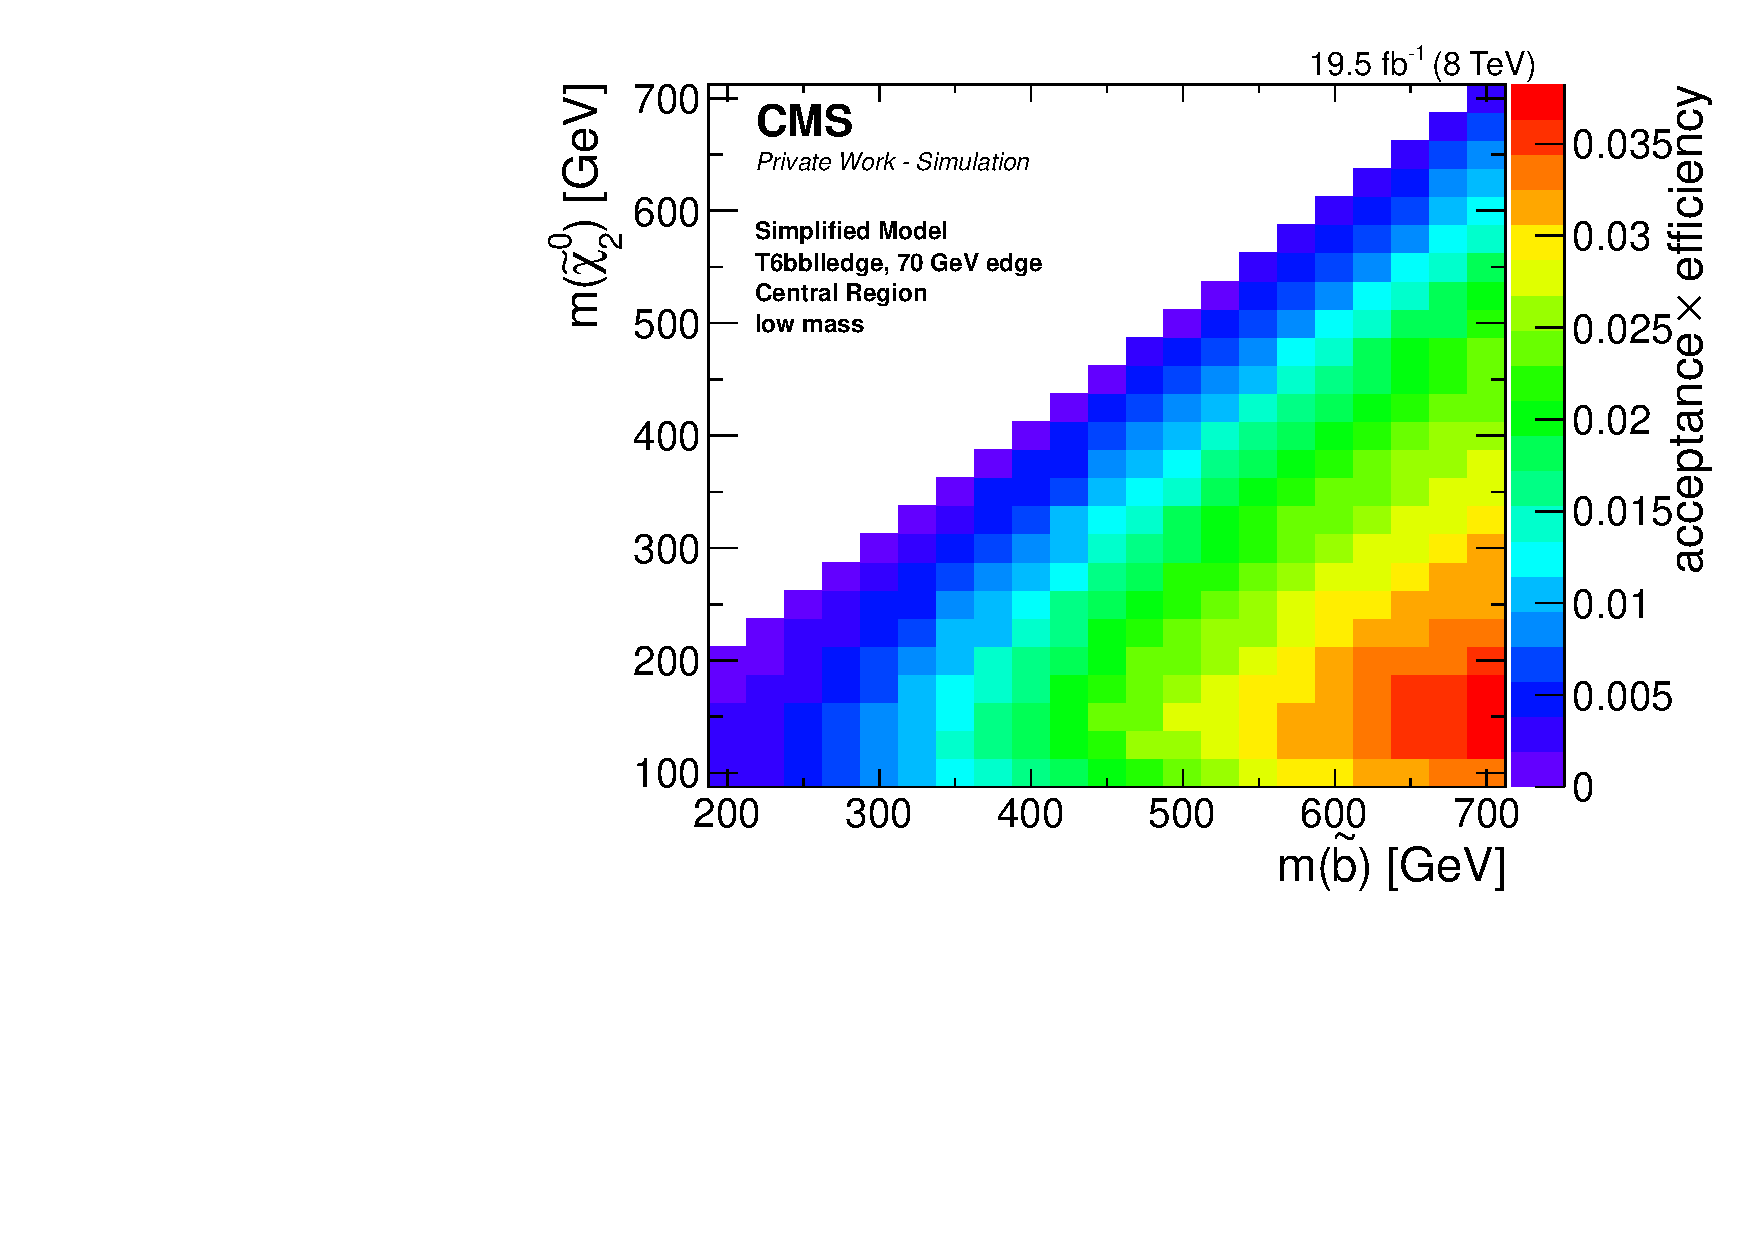
\includegraphics[width=\textwidth]{plots/limits/T6bblledge_70_GeV_Edge_Barrel_lowMll_signalEfficiency.pdf}
\end{minipage}
\begin{minipage}[t]{0.49\textwidth}
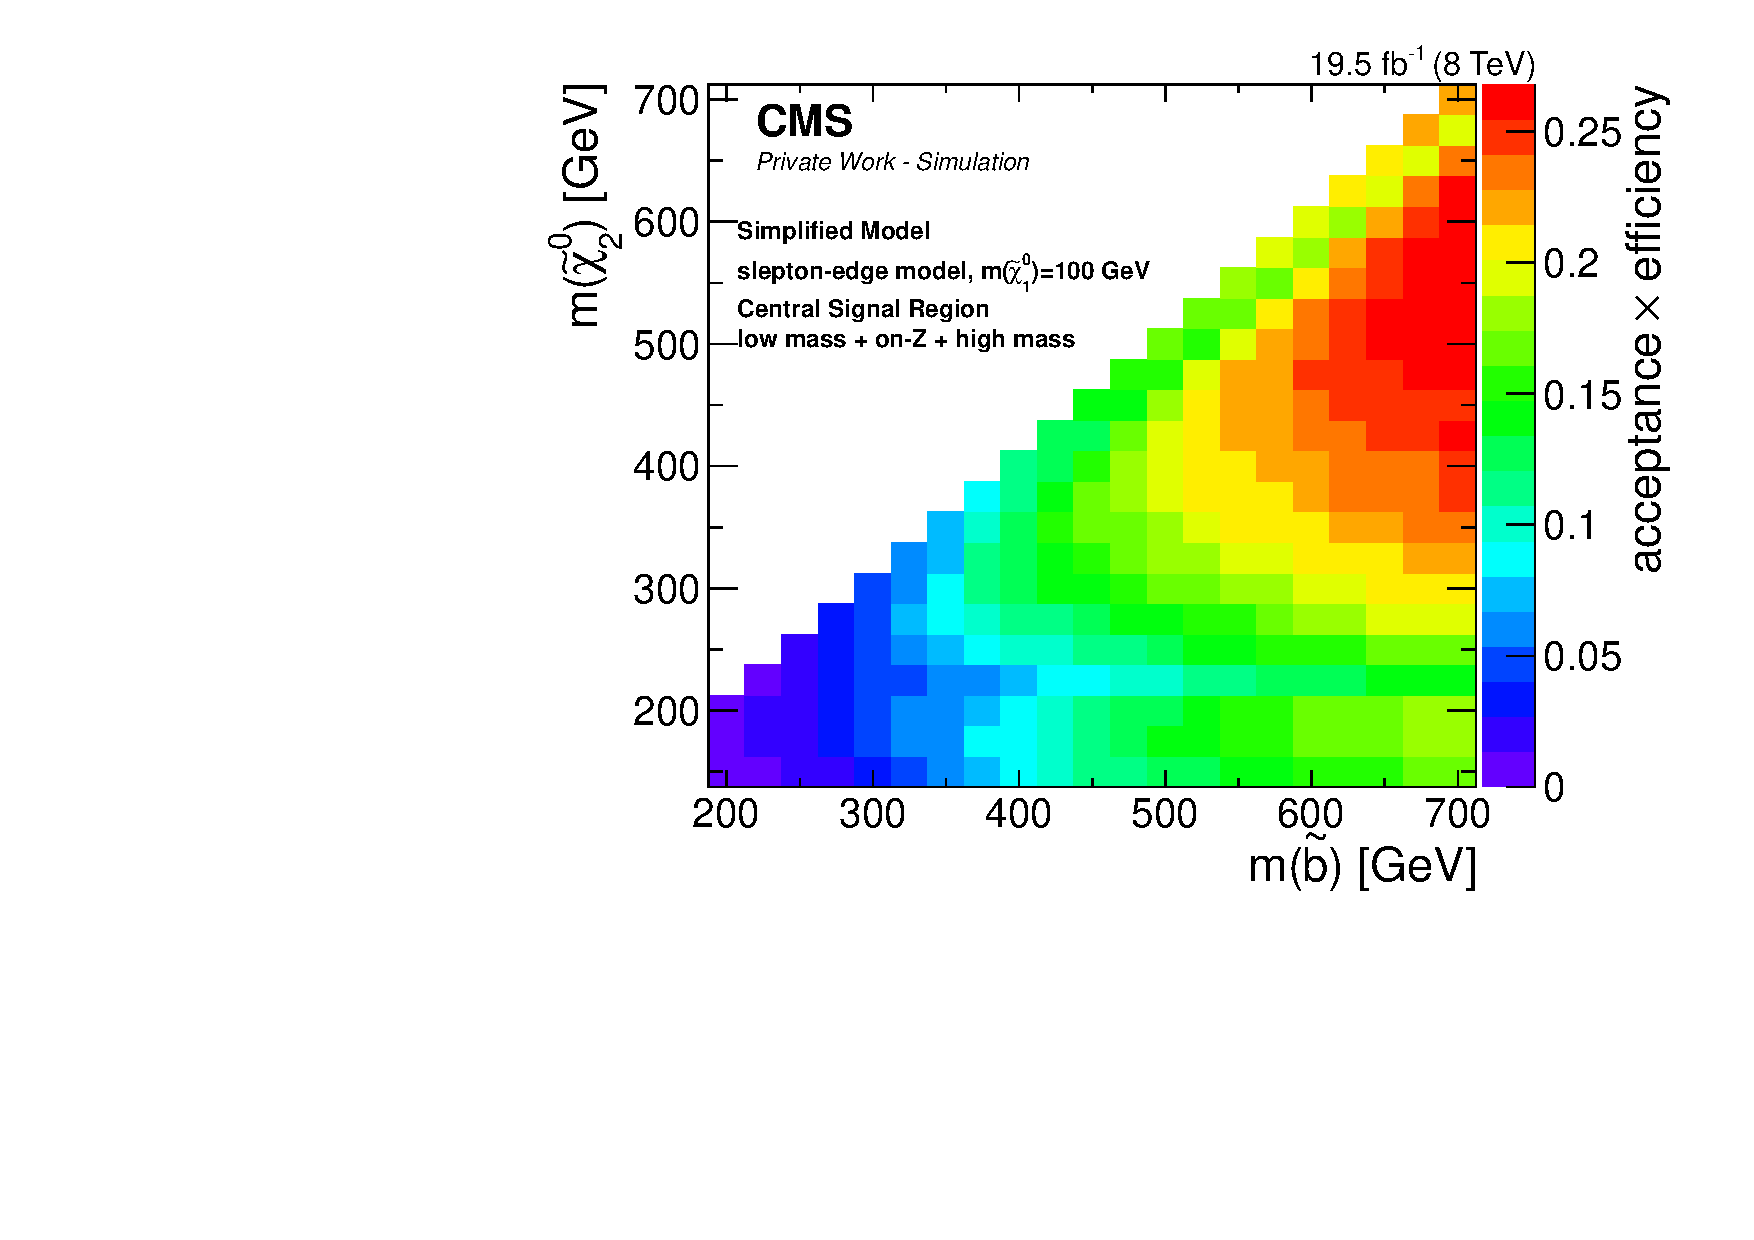
\includegraphics[width=\textwidth]{plots/limits/T6bbllslepton_m_n_1_100_Barrel_signalEfficiency_Reweighted.pdf}
\end{minipage}
\caption{Signal acceptance$\times$efficiency in the $m_{\sbottom}$-$m_{\secondchi}$ plane for the fixed-edge (left) and slepton-edge (right) model for the central signal region.}
\label{fig:sigEff}
\end{figure}
\subsubsection{Systematic uncertainties}
A variety of systematic uncertainties in the signal modelling have to taken into account. The integrated luminosity is measured with a precision of 2.6\%~\cite{CMS-PAS-LUM-13-001}. Variations of the parton distribution functions (PDF) according to the PDF4LHC recommendations~\cite{Alekhin:2011sk,Botje:2011sn,Ball:2012cx,Martin:2009iq,Lai:2010vv} result in an uncertainty of 0--6\% in the signal acceptance. Uncertainties related to lepton efficiencies are of the size of 1\% per lepton. Furthermore, the corrections of the lepton efficiency differences between fast and full detector simulation amount to another 1\% per lepton. The dilepton trigger efficiencies are measured with a precision of 5\%, as described in Section~\ref{sec:triggerEffs}. Uncertainties on the muon momentum scale have negligible impact on the signal acceptance, whereas the uncertainty in the electron energy scale is 0.6\% for central and 1.5\% for forward leptons. Jet energy scale uncertainties~\cite{1748-0221-6-11-P11002} result in an uncertainty in the signal yield of 0--8\%. The uncertainties in the modeling of the objects in the events are propagated to the \MET measurements, resulting in an uncertainty in the signal acceptance of 0--8\%. Here the contributions from the jet energy scale uncertainties are dominant. The events are corrected for difference between observed data and the modelling of initial-state-radiation (ISR) in Madgraph~\cite{Chatrchyan:2013xna} Uncertainties in these corrections are propagated to the event selection and result in an uncertainty of 0--14\% in the signal yield.
The uncertainty associated with pileup reweighting is evaluated by shifting the inelastic cross section by $\pm5\%$, resulting in an uncertainty on the signal acceptance of about 1\%. The uncertainties are summarised in Table~\ref{tab:sysUncerts}.

\begin{table}
\begin{center}
\caption{Summary of systematic uncertainties on the signal efficiency.}
\label{tab:sysUncerts}
\begin{tabular}{l|c}
Uncertainty source & Impact on signal yield [\%]\\ \hline 
Luminosity & 2.6 \\
PDFs on acceptance & 0--6 \\ 
Lepton identification/isolation & 2\\
Fast simulation lepton identification/isolation & 2 \\
Dilepton trigger & 5 \\
Lepton energy scale & 0--5  \\
\MET & 0--8  \\
Jet energy scale/resolution & 0--8  \\
ISR modeling & 0--14 \\
Additional interactions & 1 \\
%\multicolumn{2}{c}{Theoretical Uncertainties}\\
%\hline
%Fact./Renorm. Scale and PDFs& 14-18   \\
\end{tabular}
\end{center}
\end{table}
The combined systematic uncertainties are shown in Figure~\ref{fig:sys}. For the most part of the $m_{\sbottom}$-$m_{\secondchi}$ plane it ranges from 5-7\%. However, close to the diagonal this increases, caused by a larger impact of JES and ISR uncertainties. This is due to the overall lower jet \pt in this region, increasing the probability for threshold effects around the jet \pt requirement of $\unit{40}{\giga\electronvolt}$. The largest uncertainties are observed for both low masses of the \sbottom and \secondchi, exceeding 20\% for the fixed-edge model and   reaching 15\% for the slepton-edge model.
\begin{figure}[htbp]
\centering
\begin{minipage}[t]{0.49\textwidth}
  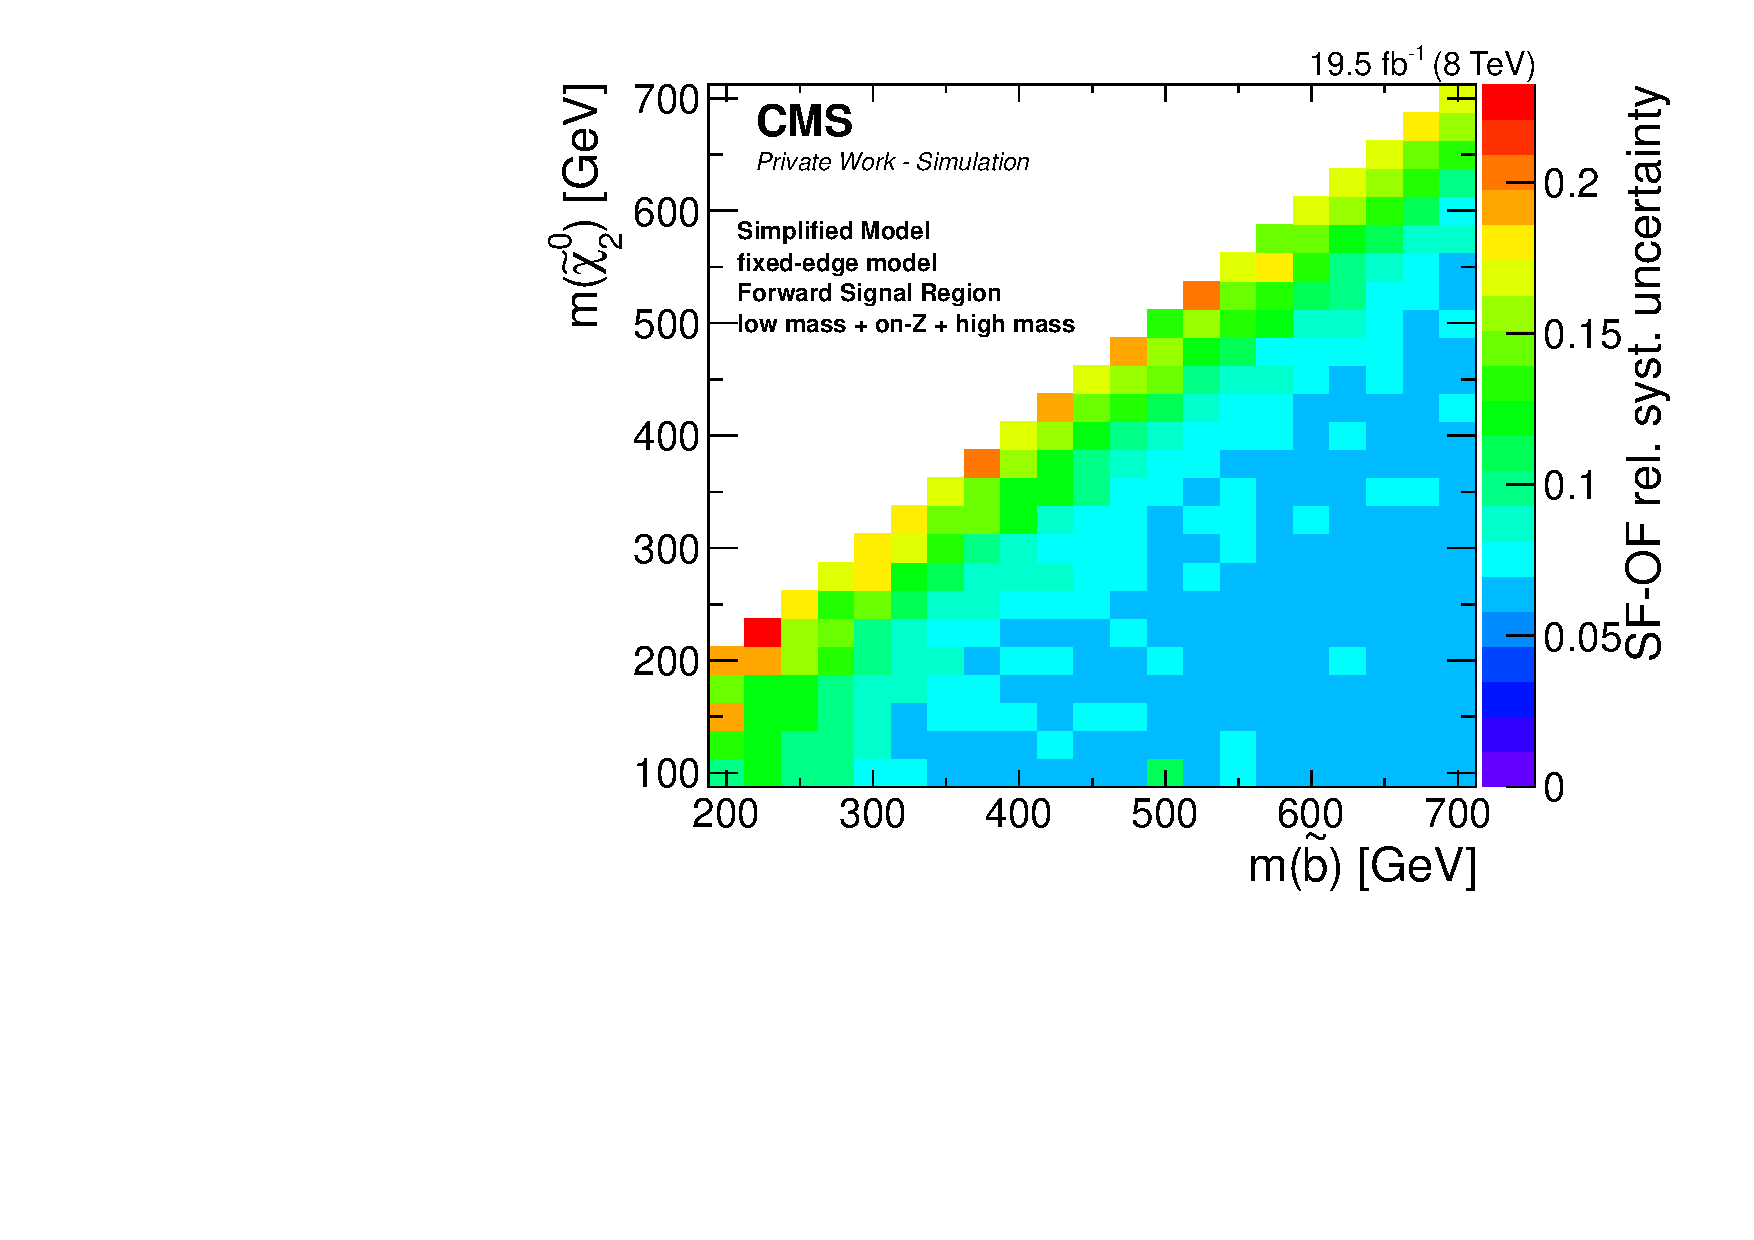
\includegraphics[width=\textwidth]{plots/limits/T6bblledge_70_GeV_Edge_Endcap_syst_err.pdf}
\end{minipage}
\begin{minipage}[t]{0.49\textwidth}
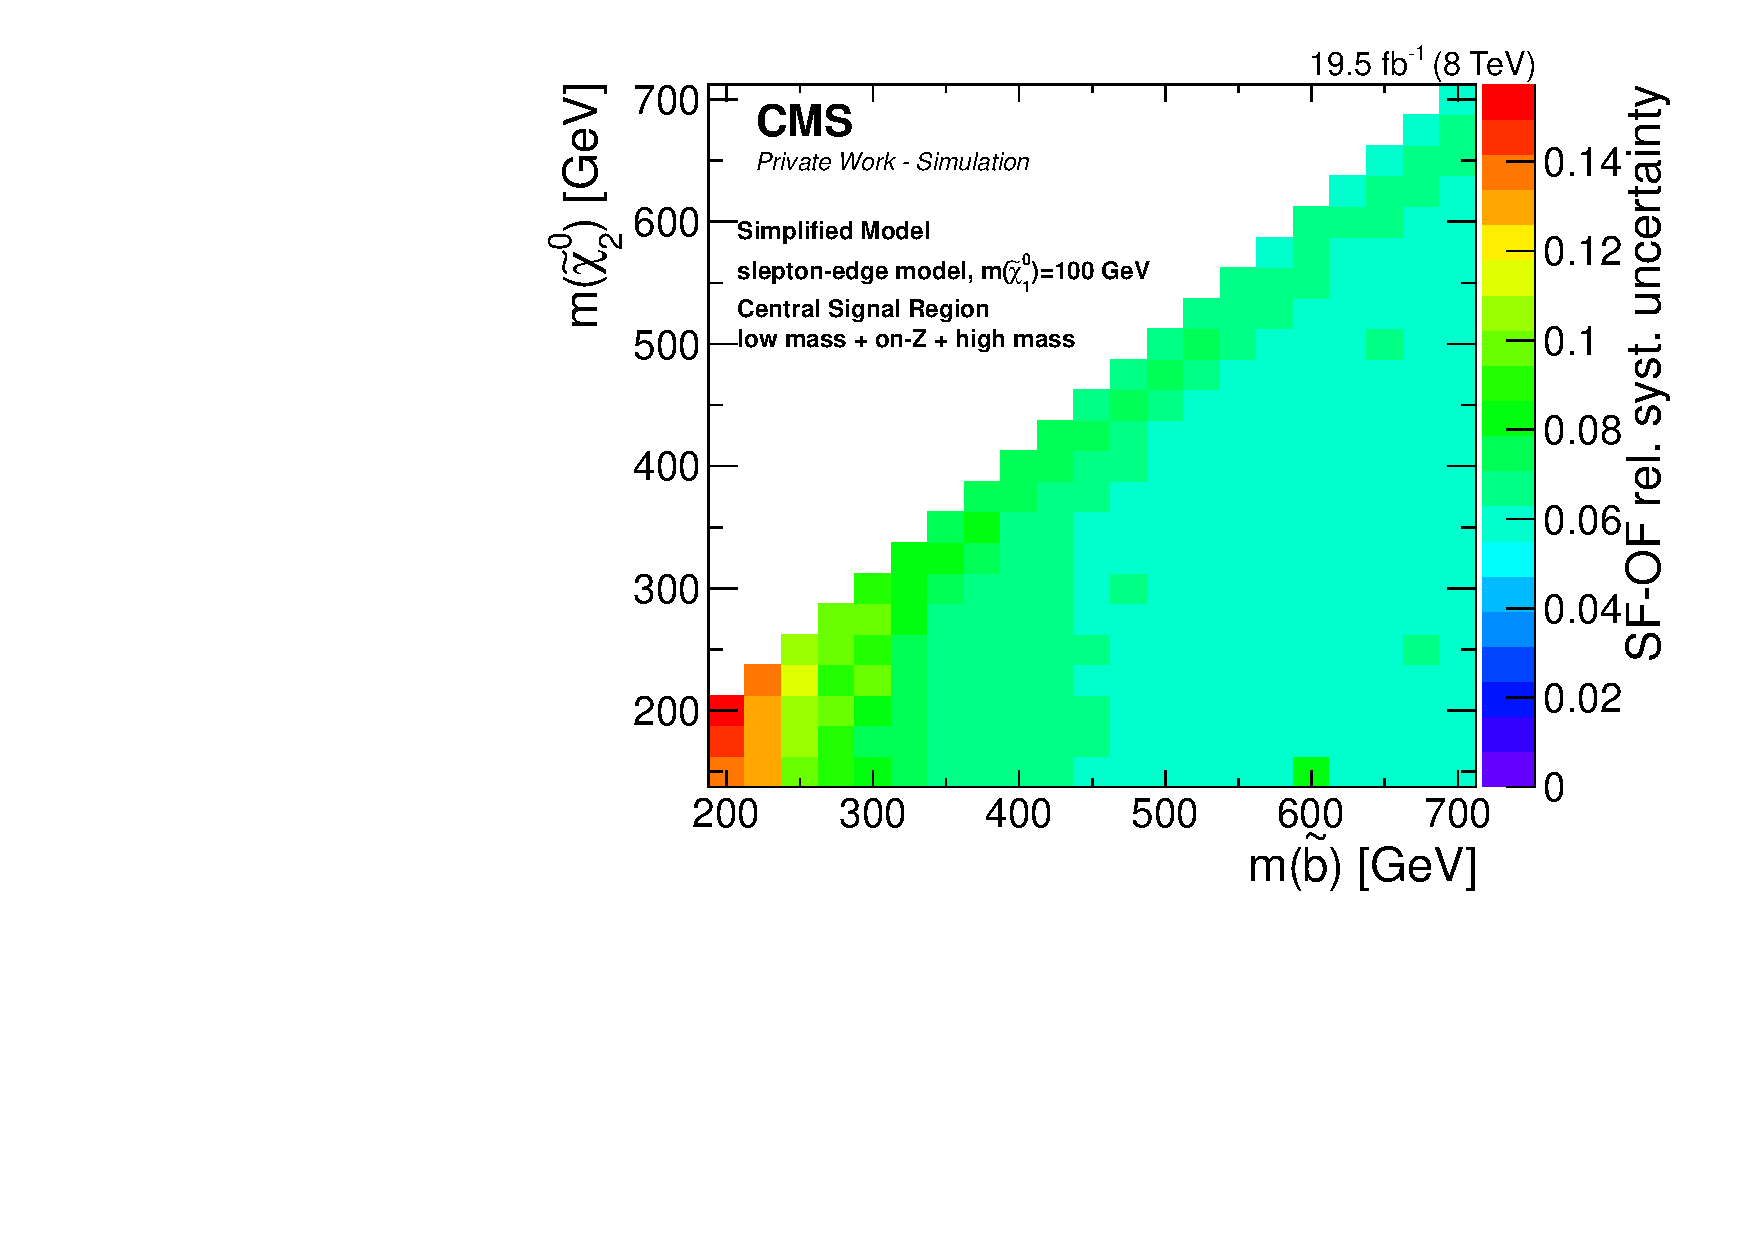
\includegraphics[width=\textwidth]{plots/limits/T6bbllslepton_m_n_1_100_Barrel_syst_err_Reweighted.pdf}
\end{minipage}
\caption{Systematic uncertainty on the signal yield in the central signal region in the $m_{\sbottom}$-$m_{\secondchi}$ plane for the fixed-edge (left) and slepton-edge (right) model.}
\label{fig:sys}
\end{figure}
\subsection{Statistical interpretation}
The results of the counting experiment are translated into exclusion limits by testing the compatibility of the signal plus background ($s+b$) and background only ($b$) hypothesis, treating each signal point in the parameter scans as a separate signal hypothesis. For this purpose, a likelihood function is defined~\cite{HiggsTool1}
\begin{equation}
\label{eq:like}
\mathcal{L}(data|\mu,\theta) = \text{Poisson}(data|\mu\cdot s(\theta) + b(\theta))\cdot p(\tilde{\theta}|\theta),
\end{equation}
where $\mu$ is a signal strength parameter, $\mu = 0$ corresponding to the background only hypothesis and $\mu > 0$ to the  $s+b$ hypothesis, and $p(\tilde{\theta}|\theta)$ parametrises the nuisance parameters $\theta$, with $\tilde{\theta}$ being the nominal value of these parameters. Based on these likelihoods, a test statistic is defined utilizing a profile likelihood ratio: 
\begin{equation}
\tilde{q_{\mu}} = -2 ln\frac{\mathcal{L}(data|\mu,\hat{\theta}_\mu)}{\mathcal{L}(data|\hat{\mu},\hat{\theta})},
\end{equation}
where the $\hat{\theta}_\mu$ represent the maximum likelihood estimators for the nuisance parameters for a given $\mu$, whereas $\hat{\mu}$ and $\hat{\theta}$ indicate the global maximum of the likelihood. For the parametrisation of the nuisance parameters $p(\tilde{\theta}|\theta)$ in equation~\ref{eq:like}, log-normal distributions are chosen. The distribution of the test statistics is then sampled dicing pseudo-experiments for some $\mu > 0$ and $\mu = 0$, representing the $s+b$ and $b$ hypotheses that are tested. The p-values $p_{s+b}$ and $p_{b}$ are defined as the probability to obtain a value of the test statistics as large or larger than the one observed in data for the given hypothesis. To obtain an upper limit on the signal cross section the value of $\mu$ is chosen where $\mathrm{CL}_{\mathrm{s}} = \frac{p_{s+b}}{p_b}$ equals 0.05, corresponding to a 95\% confidence level (CL). In the calculation, all six bins of the counting experiment are combined by multiplying the likelihoods of the different channels. In this procedure, all uncertainties on both background and signal are assumed to be uncorrelated among each other but fully correlated among the different bins.

The resulting exclusion limits are shown in Figure~\ref{fig:limits}. The left plot shows the exclusion limit in the $m_{\sbottom}$-$m_{\secondchi}$ plane for the fixed-edge model. As this model is specifically tuned to provide signals consistent with the excess observed in the low-mass central signal region, the observed limit deviates from the expected one by about $\unit{75}{\giga\electronvolt}$. Given the assumption of this model, \sbottom masses up to about $\unit{375}{\giga\electronvolt}$ are excluded, depending on the mass of the \secondchi. The right plot shows the limit for the slepton-edge model. Because of the much larger branching fraction into leptons in this model, higher masses can be excluded. The expected limit reaches \sbottom masses of about $\unit{600}{\giga\electronvolt}$ roughly independent of $m_{\secondchi}$, except for the region around $m_{\secondchi} = \unit{225}{\giga\electronvolt}$, where it drops below $\unit{550}{\giga\electronvolt}$ because of the gaps in acceptance discussed above. For lower $m_{\secondchi}$ the observed limit is significantly weaker than the expected one as here the limit is dominated by the low-mass signal region in which the excess was observed. For higher $m_{\secondchi}$, the observed limit agrees with the expected one within one standard deviation. The observed lower limit on $m_{\sbottom}$ ranges from $\unit{470}{\giga\electronvolt}$ to $\unit{590}{\giga\electronvolt}$, depending on $m_{\secondchi}$.
\begin{figure}[htbp]
\centering
\begin{minipage}[t]{0.49\textwidth}
  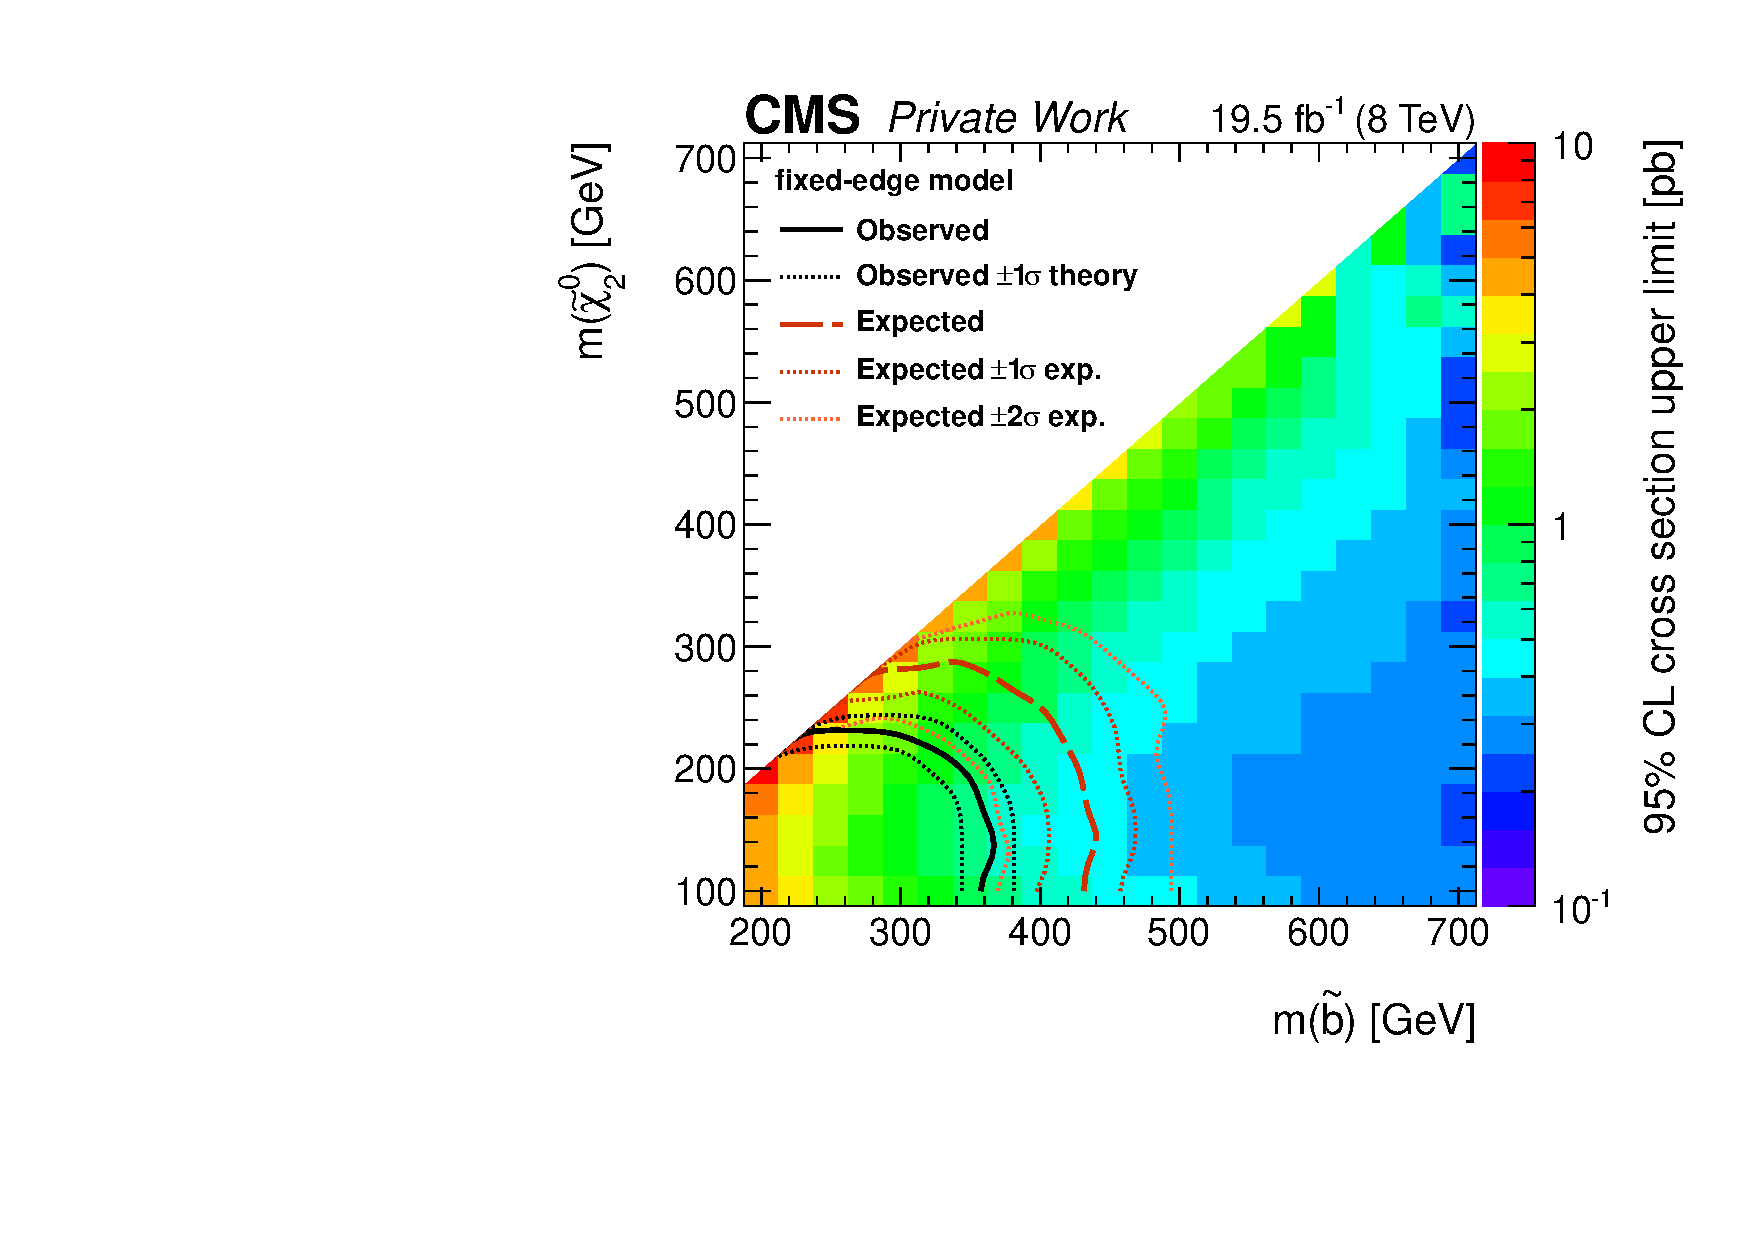
\includegraphics[width=\textwidth]{plots/limits/Fixed_Edge_sbottom_neutralino2_Exclusion_witXsecLimit.pdf}
\end{minipage}
\begin{minipage}[t]{0.49\textwidth}
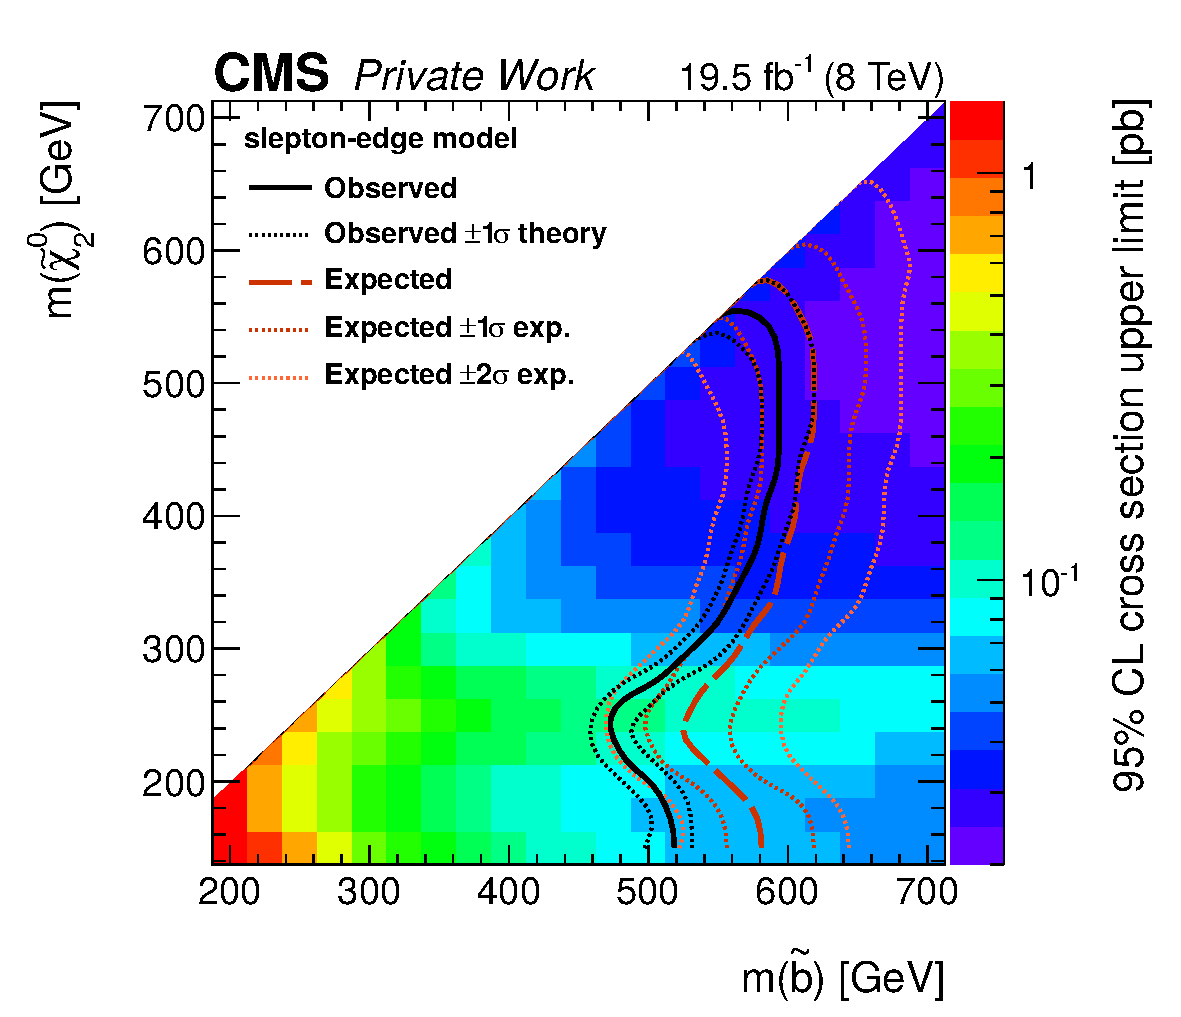
\includegraphics[width=\textwidth]{plots/limits/Fixed_Neutralino_sbottom_neutralino2_Exclusion_witXsecLimit.pdf}
\end{minipage}
\caption{Exclusion limits in the $m_{\sbottom}$-$m_{\secondchi}$ plane for the fixed-edge (left) and slepton-edge (right) model. For each signal point the upper cross section limit is shown colour coded. The intersection of the theoretical with the excluded cross section is shown as a solid black line, with every signal point to the left and below the curve being excluded. The $1-\sigma$ uncertainty interval on the observed limit is shown as dotted black lines. The expected limit together with the $1-$ and $2-\sigma$ interval are shown as brownish solid and dashed lines.}
\label{fig:limits}
\end{figure}
%\chapter{Efficiencies for \Wprime searches}
%\input{TP}
\chapter{Systematic Uncertainties}
%\input{systematics}
%\chapter{Background Estimation}
%\input{BackgroundFit}
\chapter{Statistical Interpretation}
%\input{Statistics}
\chapter{Conclusion}
%In this thesis a search for supersymmetry in final states with two same-flavour opposite-sign leptons, using full dataset of proton-proton collisions recorded by the CMS in 2012, corresponding to \lumi, has been presented. The analysis has focused on the correlated production of leptons in the decay of a neutralino, resulting in a distinct edge structure in the distribution of the invariant mass  of the lepton pairs. 

The characteristic signature of the strong production of supersymmetric particles in R-partiy convserving models, namely the presence of hadronic jets and missing transverse energy, has been exploited to separate a potential signal from the Standard Model backgrounds. The contributions of Standard Model processes to the thereby defined event selection have been estimated exclusively from the data itself. The most dominant backgrounds are symmetric in the production of same-flavour and opposite flavour lepton pairs. Therefore, the estimates for these backgrounds have been derived from the opposite-flavour event sample. Corrections for efficiency effects were derived using two independent methods and taken into account in these estimates, for which a precision of 5-10\% have been achieved.  The validity of this approach has been established using both data and simulated events. 

In search of edges in the dilepton mass distribtuon, shape information have been used by performing an unbinned maximum likelihood fit to both the same-flavour and opposite-flavour event samples. The fit consists of parametrisations for flavour-symmetric and Drell--Yan background and a triangular signal model. The best fit is found including a signal contribution with an endpoint of the signal shape of $\unit{82.4^{+2.1}_{-3.3}}{\giga\electronvolt}$ and signal yields of $140\pm44$ events for events where both leptons are reconstructed in the central part of the CMS detector and $2\pm22$ events for events where at least one of the leptons is located in the one of the endcaps. The observed effect corresponds to a local significance of $2.5\,\sigma$, which reduces to $1.7\,\sigma$ is the probability to observe an equal or large effect anywhere in the considered mass range is taken into account. 

In a second approach event yields are compared to the background estimates in six region of dilepton mass and lepton pseudorapidity. They are found to be consistent with each other except in the mass range $\unit{20}{\giga\electronvolt} < \mll < \unit{70}{\giga\electronvolt}$, where an excess of $109\pm48$ events is observed, corresponding to a local significance of $2.2\,\sigma$. The results of this approach are found to be consistent with the fit. 

The properties of the events in the excess differ not significantly from those of the backgrounds. No systematic effects responsible for the observation have been found. The development of the effect over time shows that it is only present in roughly the first half of the recorded data. 

As no clear hint for the presence of supersymmetry has been observed, exclusion limits are set in two simplified models which simulate the pair production of bottom squarks. These models contain the decay $\secondchi \rightarrow \firstchi \ell\ell$ either via an off-shell \Z boson (fixed-edge model) or via both sleptons or on- and off-shell \Z bosons (slepton-edge model). In the first model, \sbottom masses up to $\unit{375}{\giga\electronvolt}$ have been exluded, depending on the mass of the \secondchi. In the second model, in which the branching ratio into lepton pairs is much higher, the limit ranges from $\unit{470}{\giga\electronvolt}$ to $\unit{590}{\giga\electronvolt}$, again depending on $m_{\secondchi}$. 

At the time of writing this thesis, the Large Hadron Collider has begun the commissioning of the machine for the next run at  an increased centre-of-mass energy of $\unit{13}{\tera\electronvolt}$. After two years of shut-down, new data is eagerly awaited and preparations are ongoing for the analysis of the new dataset. The expected integrated luminosity for 2015 of about $10\,\mathrm{fb}^{-1}$ will probably not be sufficient to reach the same sensitivity of the analysis presented here. Nevertheless it is expected to provide an indication if the observed excess in the 2012 dataset might have been a first hint of a signal for new physics after all. 

%\input{appendix}
%\bibliographystyle{abbrv}
\bibliographystyle{unsrt}
\bibliography{thesis.bib}
%\input{Literature}

%\input{Erkl�rung}
%\input{Danksagung}


\end{document}